\begin{enumerate}[label=\thechapter.\arabic*,ref=\thechapter.\theenumi]
\item The network shown below has a resonant frequency of 150 kHz and bandwidth of 600
Hz. The Q-factor of the network is \rule{1cm}{0.15mm}\\
(rounded off to one decimal place).\\
\hfill(GATE 2022 EC)\\
\begin{figure}[ht]
  \centering
  
      \begin{circuitikz}[american]
    \draw (0,0) to [short, *-] (5,0) to [R=R] (5,2) to [L=L] (5,4) to [short] (2,4) to [C=C] (2,0);
    \draw (0,4) to [short, *-] (2,4);
\end{circuitikz}
  
  \caption{Circuit 1}
\end{figure}\\
\solution\\
\iffalse
\documentclass[journal,12pt,twocolumn]{IEEEtran}
\usepackage{amsmath,amssymb,amsfonts,amsthm}
\usepackage{txfonts}
\usepackage{tkz-euclide}
\usepackage{listings}
\usepackage{gvv}
\usepackage[latin1]{inputenc}
\usepackage{adjustbox}
\usepackage{array}
\usepackage{tabularx}
\usepackage{enumitem}
\usepackage{pgf}
\usepackage{lmodern}
\usepackage{circuitikz}
\usepackage{tikz}
\usepackage{graphicx}


\begin{document}
\bibliographystyle{IEEEtran}

\vspace{3cm}

\title{}
\author{EE23BTECH11054 -  Sai Krishna Shanigarapu$^{*}$
}
\maketitle
\newpage
\bigskip

\section*{Gate EE 2022}
28. \hspace{2pt}The network shown below has a resonant frequency of 150 kHz and bandwidth of 600
Hz. The Q-factor of the network is \rule{1cm}{0.15mm}\\
(rounded off to one decimal place).\\
\hfill(GATE 2022 EC)\\
\begin{figure}[ht]
  \centering
  
      \begin{circuitikz}[american]
    \draw (0,0) to [short, *-] (5,0) to [R=R] (5,2) to [L=L] (5,4) to [short] (2,4) to [C=C] (2,0);
    \draw (0,4) to [short, *-] (2,4);
\end{circuitikz}
  
  \caption{Circuit 1}
\end{figure}\\
\solution
\fi

\begin{figure}[ht]
  \centering
  
      \begin{circuitikz}[american]
    \draw (0,0) to [short, *-] (5,0) to [R=R] (5,2) to [L=$j\omega L$] (5,4) to [short] (2,4) to [C=$\frac{1}{j\omega C}$] (2,0);
    \draw (0,4) to [short, *-] (2,4);
\end{circuitikz}

  \caption{Circuit 2}
\end{figure}


\begin{table}[ht]
    \centering
 
    \setlength{\arrayrulewidth}{0.3mm}
\setlength{\tabcolsep}{20pt}
\renewcommand{\arraystretch}{1.3}


\begin{tabular}{|c|c|c|}
\hline
Parameter & Description & Value\\
\hline
$f_0$ & Resonant frequency & 150 kHz\\
\hline
$B$ & Bandwidth & 600 Hz\\
\hline
\end{tabular}

    \caption{Parameters}
    \label{tab:tab1_gate_ee_2022_28_054}
\end{table}

\begin{table}[ht]
    \centering

    \setlength{\arrayrulewidth}{0.3mm}
\setlength{\tabcolsep}{20pt}
\renewcommand{\arraystretch}{1.5}


\begin{tabular}{|c|c|c|}
\hline
Parameter & Description & Formula\\
\hline
$Q$ & Quality factor & $\frac{X_L}{R}$\\
\hline
$B$ & Bandwidth & $\frac{R}{2 \pi L}$\\
\hline
$\omega_0$ & Radial resonant frequency & $2 \pi f_0$\\
\hline
$X_L$ & Inductive reactance & $\omega L$\\
\hline
$X_C$ & Capacitive reactance & $\frac{1}{\omega C}$\\
\hline

\end{tabular}


    \caption{Formulae}
    \label{tab:tab2_gate_ee_2022_28_054}
\end{table}

At Resonance, 
\begin{align}
    X_L & = X_C\\
    \omega_0 L &= \frac{1}{\omega_0 C}\\
    \omega_0 &= \frac{1}{\sqrt{LC}}\\
    2 \pi f_0 &= \frac{1}{\sqrt{LC}}\\
    \implies f_0 &= \frac{1}{2 \pi \sqrt{LC}} \label{eq:eq1_gate_ee_2022_28_054}    
\end{align}

Using Table \ref{tab:tab2_gate_ee_2022_28_054},
\begin{align}
    Q &= \frac{X_L}{R}\\
    &= \frac{\omega_0 L}{R}\\
    &= \brak{\frac{1}{\sqrt{LC}}}\frac{L}{R}\\
    \implies Q &= \frac{1}{R}\sqrt{\frac{L}{C}} \label{eq:eq2_gate_ee_2022_28_054}
\end{align}

From eq (\ref{eq:eq1_gate_ee_2022_28_054}) and Table \ref{tab:tab2_gate_ee_2022_28_054}
\begin{align}
    \frac{f_0}{B} &= \brak{\frac{1}{2\pi \sqrt{LC}}}\frac{2 \pi L}{R}\\
    &= \brak{\frac{1}{\sqrt{LC}}}\frac{L}{R}\\
    \implies \frac{f_0}{B} &= \frac{1}{R}\sqrt{\frac{L}{C}} \label{eq:eq3_gate_ee_2022_28_054}
\end{align}

From Table \ref{tab:tab1_gate_ee_2022_28_054}, eq (\ref{eq:eq2_gate_ee_2022_28_054}) and eq (\ref{eq:eq3_gate_ee_2022_28_054}),
\begin{align}
    Q &= \frac{f_0}{B}\\
     &=\frac{150 \text{ x } 10^3}{600}\\
    &= 250
\end{align}

$\therefore$ Q-factor is 250

\begin{figure}[ht]
    \centering
    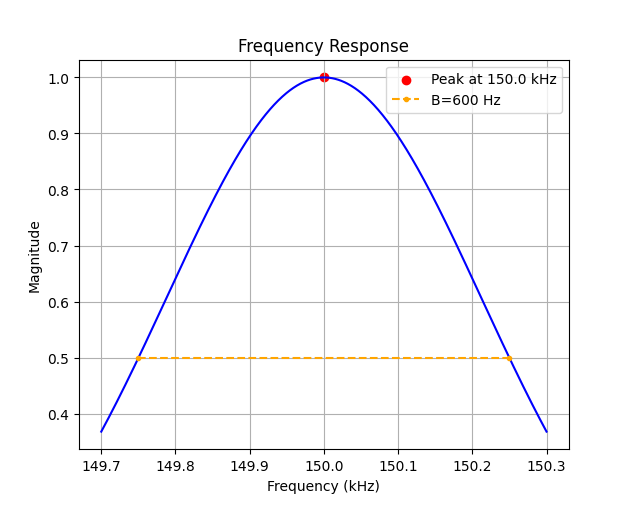
\includegraphics[width=\columnwidth]{2022/EE/28/figs/Figure_1.png}
    \caption{Plot of Q-factor}
    \label{fig:fig1_gate_ee_2022_18_054}
\end{figure}

%\end{document}

\pagebreak
\item A circuit with an ideal OPAMP is shown. The Bode plot for the magnitude (in dB)
 of the gain transfer function $ \brak{A \brak{j \omega}} = \dfrac{ V_{out}\brak{j \omega}}{V_{in}\brak{j \omega}}$ of the circuit is also
provided (here, $\omega$ is the angular frequency in $ rad/s $). The values of $R$ and $C$ are 
\begin{figure}[ht]
	\centering
    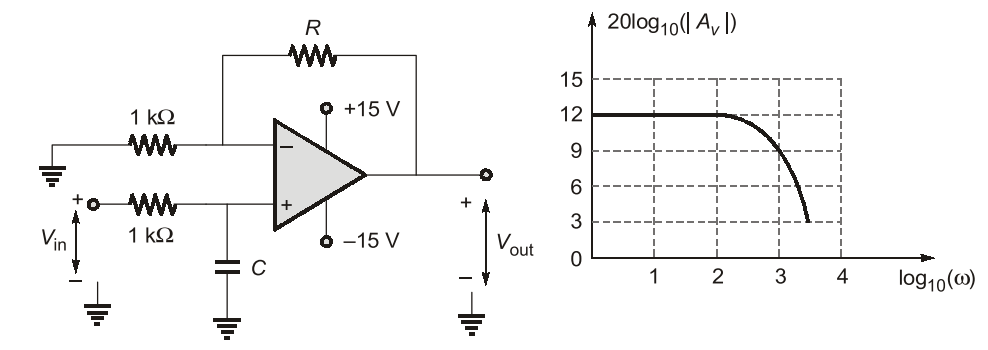
\includegraphics[width=\columnwidth]{2022/EC/42/figs/fig1.png}
    \label{fig:2022.42.39}
\end{figure} 
\begin{enumerate}[label = (\Alph*)]
     \item $R$ = $3k\ohm$,  $C$ = $1\mu F$\\
     \item $R$ = $1k\ohm$,  $C$ = $3\mu F$\\
     \item $R$ = $4k\ohm$,  $C$ = $1\mu F$\\
     \item $R$ = $3k\ohm$,  $C$ = $2\mu F$\\
\end{enumerate}
\hfill(GATE 2022 EC)\\
\solution\\
%\iffalse
\let\negmedspace\undefined
\let\negthickspace\undefined
\documentclass[journal,12pt,twocolumn]{IEEEtran}
\usepackage{cite}
\usepackage{amsmath,amssymb,amsfonts,amsthm}
\usepackage{algorithmic}
\usepackage{graphicx}
\usepackage{textcomp}
\usepackage{xcolor}
\usepackage{txfonts}
\usepackage{listings}
\usepackage{enumitem}
\usepackage{mathtools}
\usepackage{gensymb}
\usepackage{comment}
\usepackage[breaklinks=true]{hyperref}
\usepackage{tkz-euclide} 
\usepackage{listings}
\usepackage{gvv}  
\usepackage{tikz}
\usepackage{circuitikz} 
\usepackage{caption}

\def\inputGnumericTable{}                                
\usepackage[latin1]{inputenc}                 
\usepackage{color}                            
\usepackage{array}                            
\usepackage{longtable}                        
\usepackage{calc}                            
\usepackage{multirow}                      
\usepackage{hhline}                           
\usepackage{ifthen}                          
\usepackage{lscape}
\usepackage{amsmath}
\newtheorem{theorem}{Theorem}[section]
\newtheorem{problem}{Problem}
\newtheorem{proposition}{Proposition}[section]
\newtheorem{lemma}{Lemma}[section]
\newtheorem{corollary}[theorem]{Corollary}
\newtheorem{example}{Example}[section]
\newtheorem{definition}[problem]{Definition}
\newcommand{\BEQA}{\begin{eqnarray}}
\newcommand{\EEQA}{\end{eqnarray}}
\newcommand{\define}{\stackrel{\triangle}{=}}
\theoremstyle{remark}
\newtheorem{rem}{Remark}


\begin{document}
%

\bibliographystyle{IEEEtran}


\vspace{3cm}

\title{
%	\logo{
GATE 2022 EC\\
\large{EE:1205 Signals and System}

Indian Institute of Technology, Hyderabad
%	}
}
\author{Prashant Maurya

EE23BTECH11218
}	
%\title{
%	\logo{Matrix Analysis through Octave}{\begin{center}\includegraphics[scale=.24]{tlc}\end{center}}{}{HAMDSP}
%}


% paper title
% can use linebreaks \\ within to get better formatting as desired
%\title{Matrix Analysis through Octave}
%
%
% author names and IEEE memberships
% note positions of commas and nonbreaking spaces ( ~ ) LaTeX will not break
% a structure at a ~ so this keeps an author's name from being broken across
% two lines.
% use \thanks{} to gain access to the first footnote area
% a separate \thanks must be used for each paragraph as LaTeX2e's \thanks
% was not built to handle multiple paragraphs
%

%\author{<-this % stops a space
%\thanks{}}
%}
% note the % following the last \IEEEmembership and also \thanks - 
% these prevent an unwanted space from occurring between the last author name
% and the end of the author line. i.e., if you had this:
% 
% \author{....lastname \thanks{...} \thanks{...} }
%                     ^------------^------------^----Do not want these spaces!
%
% a space would be appended to the last name and could cause every name on that
% line to be shifted left slightly. This is one of those "LaTeX things". For
% instance, "\textbf{A} \textbf{B}" will typeset as "A B" not "AB". To get
% "AB" then you have to do: "\textbf{A}\textbf{B}"
% \thanks is no different in this regard, so shield the last } of each \thanks
% that ends a line with a % and do not let a space in before the next \thanks.
% Spaces after \IEEEmembership other than the last one are OK (and needed) as
% you are supposed to have spaces between the names. For what it is worth,
% this is a minor point as most people would not even notice if the said evil
% space somehow managed to creep in.



% The paper headers
%\markboth{Journal of \LaTeX\ Class Files,~Vol.~6, No.~1, January~2007}%
%{Shell \MakeLowercase{\textit{et al.}}: Bare Demo of IEEEtran.cls for Journals}
% The only time the second header will appear is for the odd numbered pages
% after the title page when using the twoside option.
% 
% *** Note that you probably will NOT want to include the author's ***
% *** name in the headers of peer review papers.                   ***
% You can use \ifCLASSOPTIONpeerreview for conditional compilation here if
% you desire.




% If you want to put a publisher's ID mark on the page you can do it like
% this:
%\IEEEpubid{0000--0000/00\$00.00~\copyright~2007 IEEE}
% Remember, if you use this you must call \IEEEpubidadjcol in the second
% column for its text to clear the IEEEpubid mark.



% make the title area
\maketitle

\newpage

%\tableofcontents

\bigskip

\renewcommand{\thefigure}{\arabic{figure}}
\renewcommand{\thetable}{\arabic{table}}
%\renewcommand{\theequation}{\theenumi}

%\begin{abstract}
%%\boldmath
%In this letter, an algorithm for evaluating the exact analytical bit error rate  (BER)  for the piecewise linear (PL) combiner for  multiple relays is presented. Previous results were available only for upto three relays. The algorithm is unique in the sense that  the actual mathematical expressions, that are prohibitively large, need not be explicitly obtained. The diversity gain due to multiple relays is shown through plots of the analytical BER, well supported by simulations. 
%
%\end{abstract}
% IEEEtran.cls defaults to using nonbold math in the Abstract.
% This preserves the distinction between vectors and scalars. However,
% if the journal you are submitting to favors bold math in the abstract,
% then you can use LaTeX's standard command \boldmath at the very start
% of the abstract to achieve this. Many IEEE journals frown on math
% in the abstract anyway.

% Note that keywords are not normally used for peerreview papers.
%\begin{IEEEkeywords}
%Cooperative diversity, decode and forward, piecewise linear
%\end{IEEEkeywords}



% For peer review papers, you can put extra information on the cover
% page as needed:
% \ifCLASSOPTIONpeerreview
% \begin{center} \bfseries EDICS Category: 3-BBND \end{center}
% \fi
%
% For peerreview papers, this IEEEtran command inserts a page break and
% creates the second title. It will be ignored for other modes.
%\IEEEpeerreviewmaketitle	
\textbf{Question 42:}
 A circuit with an ideal OPAMP is shown. The Bode plot for the magnitude (in dB)
 of the gain transfer function $ \brak{A \brak{j \omega}} = \dfrac{ V_{out}\brak{j \omega}}{V_{in}\brak{j \omega}}$ of the circuit is also
provided (here, $\omega$ is the angular frequency in $ rad/s $). The values of $R$ and $C$ are 
\begin{figure}[ht]
	\centering
    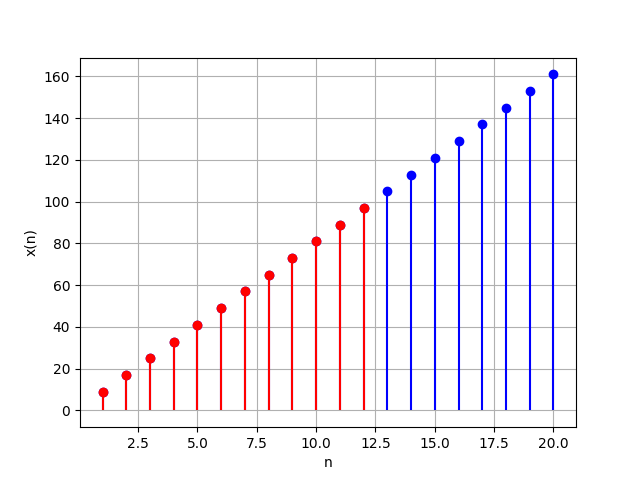
\includegraphics[width=\columnwidth]{figs/fig1.png}
    \label{fig: 1}
\end{figure}
\begin{enumerate}[label = (\Alph*)]
     \item $R$ = $3k\ohm$,  $C$ = $1\mu F$\\
     \item $R$ = $1k\ohm$,  $C$ = $3\mu F$\\
     \item $R$ = $4k\ohm$,  $C$ = $1\mu F$\\
     \item $R$ = $3k\ohm$,  $C$ = $2\mu F$\\
\end{enumerate}
\textbf{Solution}

\begin{table}[!h]
	\centering
	\begin{tabular}{|c|c|c|}
\hline
    Parameter & Description & Value\\
    \hline
    $P(s)$ & Plant Transfer Function & $\frac{0.001}{s\brak{\frac{s}{0.5}+1}\brak{\frac{s}{100}+1}}$\\
    \hline
    $C(s)$ & Lag Compensator  & $\frac{100\brak{\frac{s}{10}+1}}{\frac{s}{0.1}+1}$\\
    \hline
    $T(s)$ & Loop gain  & $P(s) C(s)$ \\
    \hline
    $\omega$ & Angular Frequency & 3rad/s \\
    \hline
\end{tabular}

	\vspace{6 pt}
	\caption{Given Parameters}
	\label{tab:enter-label}
\end{table}

\begin{figure}[ht]
	\centering
    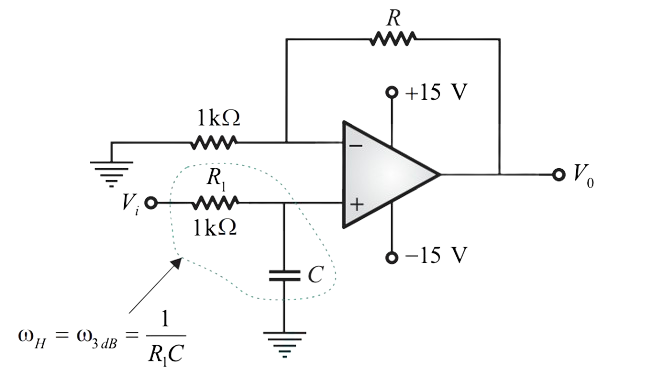
\includegraphics[width=\columnwidth]{figs/fig2.png}
    \caption{Active Low Pass Filter}
    \label{fig: 1}
\end{figure}
On applying KVL,
\begin{align}
\label{eqn:1}sR_1i_1\brak{s} +\dfrac{i_1\brak{s}}{C}=& V_{IN}\brak{s}s
\end{align}
\begin{align}
\label{eqn:2}\dfrac{i_1\brak{s}}{C} - sRi_2\brak{s} =& sV_0\brak{s}
\end{align}
From \eqref{eqn:1} and \eqref{eqn:2},
\begin{align}
\label{eqn:3} \dfrac{sV_{IN}\brak{s}}{sR_1 C+1} - sRi_2\brak{s} =& sV_0\brak{s}
\end{align}
\begin{align}
\label{eqn:4} -\dfrac{i_1\brak{s}}{C}=& sR_1i_2\brak{s}
\end{align}
From \eqref{eqn:1}, \eqref{eqn:2} and \eqref{eqn:4} ,
\begin{align}
V_{OUT}\brak{s} =& \dfrac{1+10^{-3}R}{1+sC10^3}V_{IN}\brak{s}
\end{align}
\begin{figure}[ht]
	\centering
    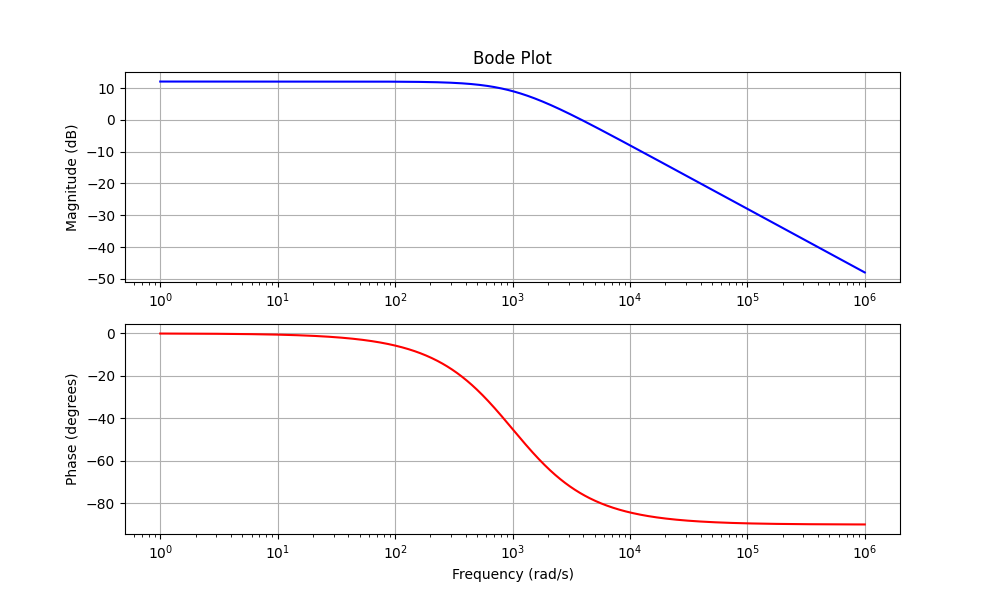
\includegraphics[width=\columnwidth]{figs/fig5.png}
    \caption{bode plot}
    \label{fig: 2}
\end{figure}
\vspace{2cm}

The 3-dB frequency from bode magnitude plot,
\begin{align}
\implies \omega_{3dB} =& 1000 \: rad/sec 
\end{align}
\begin{align}
\omega_{3dB} =& \dfrac{1}{R_1 C}\\
\implies C =& 1\mu F  
\end{align}
\begin{align}
\implies A\brak{s} =& \dfrac{V_{OUT}\brak{s}}{V_{IN}\brak{s}}\\
  		  =& \dfrac{1+10^{-3}R}{1+sC10^3}\\		
  	   |A\brak{s}| =& \dfrac{1+10^{-3}R}{\sqrt{1+\omega^210^{-6}}}	\\
\end{align}
$A_V$ at low frequency,
\begin{align}
|A_V| =& 1+ 10^{-3}R \\
1+ 10^{-3}R =& 10^{\dfrac{3}{5}}\\
R =& 3k\ohm
\end{align}
Hence, The correct option is \brak{A}.
\end{document}
\pagebreak

\item  In the circuit shown, the load is driven by a sinusoidal A.C. voltage source $V_1 = 100\angle0\degree V$ at $50Hz$. Given $R_1 = 20\Omega$, $C_1 = \brak{\frac{1000}{\pi}}\mu F$, $L_1 = \brak{\frac{20}{\pi}}mH$ and $R_2 = 4\Omega$, the power factor is \_\_\_\_\_ (round off to one decimal place)\\
\hfill(GATE 2022 IN Q52)
\begin{figure}[!h]
    \centering
    \begin{circuitikz}
        \draw(0, 0) to[sV, l = $V_1$](0, -4);
        \draw(0, -4) to [R, l = $R_2$](6, -4);
        \draw(6, 0) to[L, l = $L_1$](6, -4);
        \draw(0, 0) -- (2, 0);
        \draw(4, 0) -- (6, 0);
        \draw(2, 0.75) -- (2, -0.75);
        \draw(4, 0.75) -- (4, -0.75);

        \draw(2, 0.75) to [R, l = $R_1$](4, 0.75);
        \draw(2, -0.75) to [C, l_ = $C_1$](4, -0.75);
    \end{circuitikz}
    \caption{}
    \label{fig:1_gate.22.in.52}
\end{figure}

\solution
\iffalse
\let\negmedspace\undefined
\let\negthickspace\undefined
\documentclass[journal,12pt,twocolumn]{IEEEtran}
\usepackage{cite}
\usepackage{amsmath,amssymb,amsfonts,amsthm}
\usepackage{algorithmic}
\usepackage{graphicx}
\usepackage{textcomp}
\usepackage{xcolor}
\usepackage{txfonts}
\usepackage{listings}
\usepackage{enumitem}
\usepackage{mathtools}
\usepackage{gensymb}
\usepackage{comment}
\usepackage[breaklinks=true]{hyperref}
\usepackage{tkz-euclide} 
\usepackage{listings}
\usepackage{gvv}                            \usepackage{tikz}
\usepackage{circuitikz}
\def\inputGnumericTable{}                                
\usepackage[latin1]{inputenc}                            
\usepackage{color}                      \usepackage{gensymb}
\usepackage{array}                                       
\usepackage{longtable}                                   
\usepackage{calc}                              
\usepackage{tikz}
\usepackage{multirow}                                    
\usepackage{hhline}                                      
\usepackage{ifthen}                            
\usepackage{caption}
\usepackage{lscape}
\usepackage{amsmath}
\newtheorem{theorem}{Theorem}[section]
\newtheorem{problem}{Problem}
\newtheorem{proposition}{Proposition}[section]
\newtheorem{lemma}{Lemma}[section]
\newtheorem{corollary}[theorem]{Corollary}
\newtheorem{example}{Example}[section]
\newtheorem{definition}[problem]{Definition}
\newcommand{\BEQA}{\begin{eqnarray}}
\newcommand{\EEQA}{\end{eqnarray}}
\newcommand{\define}{\stackrel{\triangle}{=}}
\theoremstyle{remark}
\newtheorem{rem}{Remark}

\begin{document}

\bibliographystyle{IEEEtran}
\vspace{3cm}

\title{GATE 2022 IN Q52}
\author{EE23BTECH11009 - AROSHISH PRADHAN$^{*}$% <-this % stops a space
}
\maketitle
\newpage
\bigskip
\textbf{Question:} In the circuit shown, the load is driven by a sinusoidal A.C. voltage source $V_1 = 100\angle0\degree V$ at $50Hz$. Given $R_1 = 20\Omega$, $C_1 = \brak{\frac{1000}{\pi}}\mu F$, $L_1 = \brak{\frac{20}{\pi}}mH$ and $R_2 = 4\Omega$, the power factor is \_\_\_\_\_ (round off to one decimal place)\\
\hfill(GATE 2022 IN Q52)
\begin{figure}[!h]
    \centering
    \begin{circuitikz}
        \draw(0, 0) to[sV, l = $V_1$](0, -4);
        \draw(0, -4) to [R, l = $R_2$](6, -4);
        \draw(6, 0) to[L, l = $L_1$](6, -4);
        \draw(0, 0) -- (2, 0);
        \draw(4, 0) -- (6, 0);
        \draw(2, 0.75) -- (2, -0.75);
        \draw(4, 0.75) -- (4, -0.75);

        \draw(2, 0.75) to [R, l = $R_1$](4, 0.75);
        \draw(2, -0.75) to [C, l_ = $C_1$](4, -0.75);
    \end{circuitikz}
    \caption{}
    \label{fig:1_gate.22.in.52}
\end{figure}


\solution
\fi
\begin{table}[!h]
    \centering
    \begin{tabular}{|c|c|c|}
    \hline
       \textbf{Symbol}  & \textbf{Value}  & \textbf{Description}\\
    \hline
       $V_1$  & $100\angle0\degree V$ & Input Voltage \\
    \hline
        $f$ & $50Hz$ & Frequency\\
    \hline
        $\omega$ & $2\pi f$ & Angular Frequency\\
    \hline
        $R_1$ & $20\Omega$ & Resistance\\
    \hline
        $R_2$ & $4\Omega$ & Resistance\\
    \hline
        $C_1$ & $\brak{\frac{1000}{\pi}}\mu F$ & Capacitance\\
    \hline
        $L_1$ & $\brak{\frac{20}{\pi}}mH$ & Inductance\\
    \hline
        $Z_{\text{eff}}$ & & Impedance\\
    \hline
        $\cos(\phi)$ & $\dfrac{\mathrm{Re}(Z_{\text{eff}})}{\abs{Z_{\text{eff}}}}$& Power Factor\\
    \hline
    \end{tabular}
    \caption{Given Parameters}
    \label{tab:1_gate.22.in.52}
\end{table}


\begin{align}
    Z_{\text{eff}} &= R_2 + j\omega L_1 + \frac{\frac{R_1}{j\omega C_1}}{R_1 + \frac{1}{j\omega C_1}}\\
    &= 4 + 2j + \frac{-200j}{20 - 10j}\\
    &= 8-6j
\end{align}
$\therefore$ Power Factor:
\begin{align}
    \cos(\phi) &= \frac{\mathrm{Re}(Z_{\text{eff}})}{\abs{Z_{\text{eff}}}}\\
    &= \frac{8}{\sqrt{8^2 + 6^2}}\\
    &= 0.8
\end{align}
\begin{figure}[!h]
    \centering
    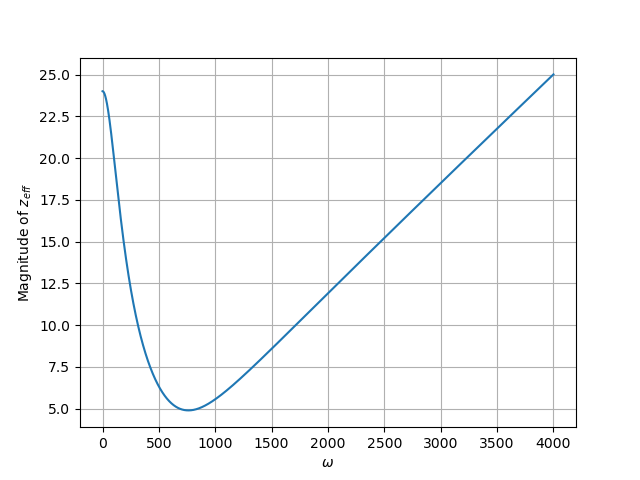
\includegraphics[width = \columnwidth]{2022/IN/52/figs/Zplot.png}
    \caption{Plot of $Z_{\text{eff}}$ vs $\omega$}
    \label{fig:2_gate.22.in.52}
\end{figure}
%\end{document}

\pagebreak

\item For the circuit shown, the locus of the impedance $ Z\brak{j\omega}$ is plotted as $ \omega$ increases from zero to infinity. The values of $ R_1$ and $ R_2$ are:
\begin{enumerate}
    \item[(A)] $ R_1 = 2\text{ k\ohm}, R_2 = 3\text{ k\ohm}$
    \item[(B)]$ R_1 = 5\text{ k\ohm}, R_2 = 2\text{ k\ohm}$
    \item[(C)] $ R_1 = 5\text{ k\ohm}, R_2 = 2.5\text{ k\ohm}$
    \item[(D)] $ R_1 = 2\text{ k\ohm}, R_2 = 5\text{ k\ohm}$
\end{enumerate}

\begin{figure}[h!]
    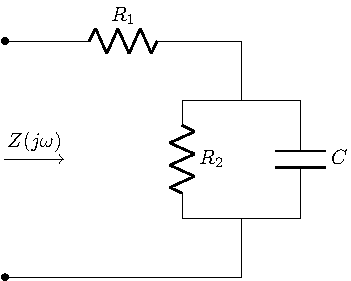
\includegraphics[width = 0.6\columnwidth]{2022/EC/38/figs/qn_fig.pdf}
    \caption{Figure of circuit}
    \centering
    \label{fig: ece38_qn_fig}
\end{figure}

\begin{figure}[h!]
    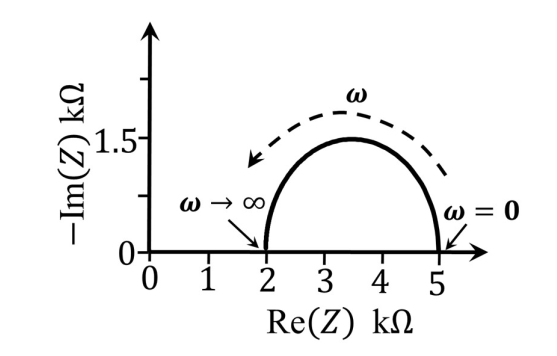
\includegraphics[width = 0.6\columnwidth]{2022/EC/38/figs/fig_2.png}
    \caption{}
    \centering
    \label{fig: ece38qn_2_fig}
\end{figure}
\hfill(GATE ECE 2022 QUESTION 38)\\
\solution
\iffalse
\let\negmedspace\undefined
\let\negthickspace\undefined
\documentclass[journal,12pt,twocolumn]{IEEEtran}
\usepackage{cite}
\usepackage{amsmath,amssymb,amsfonts,amsthm}
\usepackage{algorithmic}
\usepackage{graphicx}
\usepackage{textcomp}
\usepackage{xcolor}
\usepackage{txfonts}
\usepackage{listings}
\usepackage{enumitem}
\usepackage{mathtools}
\usepackage{gensymb}
\usepackage{comment}
\usepackage[breaklinks=true]{hyperref}
\usepackage{tkz-euclide}
\usepackage{listings}
\usepackage{gvv}
\def\inputGnumericTable{}
\usepackage[latin1]{inputenc}
\usepackage{color}
\usepackage{array}
\usepackage{longtable}
\usepackage{calc}
\usepackage{multirow}
\usepackage{hhline}
\usepackage{ifthen}
\usepackage{lscape}

\newtheorem{theorem}{Theorem}[section]
\newtheorem{problem}{Problem}
\newtheorem{proposition}{Proposition}[section]
\newtheorem{lemma}{Lemma}[section]
\newtheorem{corollary}[theorem]{Corollary}
\newtheorem{example}{Example}[section]
\newtheorem{definition}[problem]{Definition}
\newcommand{\BEQA}{\begin{eqnarray}}
\newcommand{\EEQA}{\end{eqnarray}}
\newcommand{\define}{\stackrel{\triangle}{=}}
\theoremstyle{remark}
\newtheorem{rem}{Remark}
\begin{document}

\bibliographystyle{IEEEtran}
\vspace{3cm}

\title{GATE 2022  -AE 63}
\author{EE23BTECH11057 - Shakunaveti Sai Sri Ram Varun$^{}$% &lt;-this % stops a space
}
\maketitle
\newpage
\bigskip
\vspace{2cm}
\textbf{Question: }
For the circuit shown, the locus of the impedance $ Z\brak{j\omega}$ is plotted as $ \omega$ increases from zero to infinity. The values of $ R_1$ and $ R_2$ are:
\begin{enumerate}
    \item[(A)] $ R_1 = 2\text{ k\ohm}, R_2 = 3\text{ k\ohm}$
    \item[(B)]$ R_1 = 5\text{ k\ohm}, R_2 = 2\text{ k\ohm}$
    \item[(C)] $ R_1 = 5\text{ k\ohm}, R_2 = 2.5\text{ k\ohm}$
    \item[(D)] $ R_1 = 2\text{ k\ohm}, R_2 = 5\text{ k\ohm}$
\end{enumerate}

\begin{figure}[h!]
    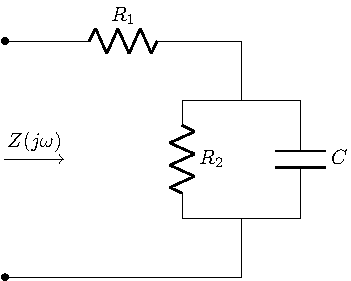
\includegraphics[width = 0.6\columnwidth]{2022/EC/38/figs/qn_fig.pdf}
    \caption{Figure of circuit}
    \centering
    \label{fig: ece38_qn_fig}
\end{figure}

\begin{figure}[h!]
    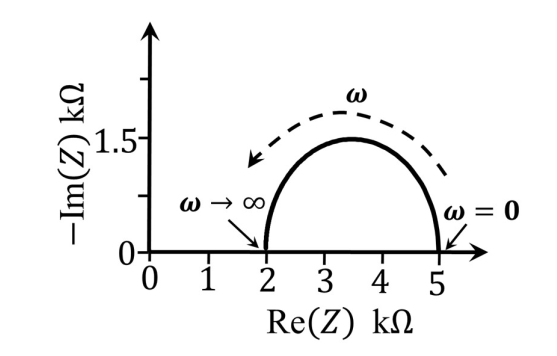
\includegraphics[width = 0.6\columnwidth]{2022/EC/38/figs/fig_2.png}
    \caption{}
    \centering
    \label{fig: ece38qn_2_fig}
\end{figure}
\hfill(GATE ECE 2022 QUESTION 38)\\
\textbf{Solution}:\\
\fi
\begin{table}[h!] 
\centering
\begin{tabular}{|c|c|c|}
    \hline
    \textbf{Parameter} & \textbf{Description} & \textbf{Value} \\
    \hline
    $ Z\brak{j\omega}$ & Impedance of circuit & ? \\
    \hline
    $ R_1$ & Resistor 1  &? \\
    \hline
    $ R_1$ & Resistor 2  &? \\
    \hline
    $ C$ & Capacitor  &? \\
    \hline
    $\omega$ & angular frequency of input voltage& $ \omega$\\
    \hline
\end{tabular}





\caption{input values}
\label{tab: Table2022ECE38}
\end{table}

In $ \omega$ domain (i.e. after Laplace transform) \figref{fig: ece38_qn_fig} can be represented as \figref{fig: ece38_ans_1_fig}
\begin{figure}[h!]
    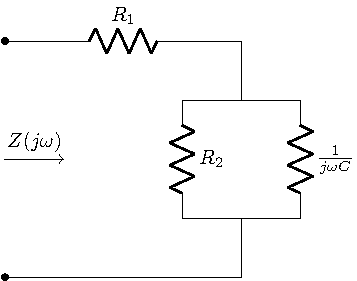
\includegraphics[width = 0.6\columnwidth]{2022/EC/38/figs/answer_fig.pdf}
    \caption{}
    \centering
    \label{fig: ece38_ans_1_fig}
\end{figure}
So, the impedance for the circuit in $ \omega$ domain is:
\begin{align}
Z\brak{j \omega} &= R_1 +  \frac{1}{\frac{1}{R_2}+ j\omega C} \label{eq: ece38_1}
\end{align}
From \figref{fig: ece38qn_2_fig}, $ Z\brak{j\omega}=2$ as $ \omega \to \infty$ and 
$ Z\brak{j\omega}=5$ as $ \omega \to 0$
\begin{align}
2 &= R_1 + \lim_{\omega\to\infty}\frac{1}{\frac{1}{R_2}+ j\omega C}\\
\implies 2 &= R_1 + \lim_{\omega\to\infty}\frac{\frac{1}{R_2}- j \omega C}{\brak{\frac{1}{R_2}}^2+ \brak{\omega C}^2}\\
\implies 2 &= R_1 + \lim_{\omega\to\infty}\frac{\frac{1}{R_2 \omega^2}- j\frac{C}{\omega}}{\brak{\frac{1}{R_2 \omega}}^2+ C^2}\\
\therefore 2\text{\ohm} &= R_1 \label{eq: ece_38_2}\\
5 &= R_1 + \frac{1}{\frac{1}{R_2}+j\brak{0}}\\
\implies 5 &= R_1 + R_2\\
\therefore 3\text{\ohm} &= R_2
\end{align}
Hence, option (A) is correct.


\pagebreak

\item In the bandpass filter circuit shown, $R_0 = 50\Omega$, $L_0 = 1 mH$, $C_0 = 10nF$. The q factor of the filter is 
\begin{figure}[h]
\renewcommand\thefigure{1}
    \centering
    \begin{circuitikz}[american]
    \draw (0,0) to [L=$L_0$, *-] (2,0) to [C=$C_0$] (4,0) to [R=$R_0$] (4,-2) to [short, -*] (0,-2);
    \draw (4,-0.3) to[short, -*] (6,-0.3);
    \draw (4,-1.7) to[short, -*] (6,-1.7);

    \node at (6,-1) {Output};
    \node at (0,-1) {Input};
    \end{circuitikz}
    \label{fig:1}
\end{figure}


\hfill(GATE 2022 IN Q33)\\
\solution
\iffalse
\let\negmedspace\undefined
\let\negthickspace\undefined
\documentclass[journal,12pt,twocolumn]{IEEEtran}
\usepackage{cite}
\usepackage{circuitikz}
\usepackage{amsmath,amssymb,amsfonts,amsthm}
\usepackage{algorithmic}
\usepackage{graphicx}
\usepackage{textcomp}
\usepackage{xcolor}
\usepackage{txfonts}
\usepackage{listings}
\usepackage{enumitem}
\usepackage{mathtools}
\usepackage{gensymb}
\usepackage{comment}
\usepackage[breaklinks=true]{hyperref}
\usepackage{tkz-euclide} 
\usepackage{listings}
\usepackage{gvv}                                        
\def\inputGnumericTable{}                                 
\usepackage[latin1]{inputenc}                                
\usepackage{color}                                            
\newtheorem{theorem}{Theorem}[section]
\usepackage{array}                                            
\usepackage{longtable}                                       
\usepackage{calc}                                             
\usepackage{multirow}                                         
\usepackage{hhline}                                           
\usepackage{ifthen}                                           
\usepackage{lscape}
\newtheorem{problem}{Problem}
\newtheorem{proposition}{Proposition}[section]
\newtheorem{lemma}{Lemma}[section]
\newtheorem{corollary}[theorem]{Corollary}
\newtheorem{example}{Example}[section]
\newtheorem{definition}[problem]{Definition}
\newcommand{\BEQA}{\begin{eqnarray}}
\newcommand{\EEQA}{\end{eqnarray}}
\newcommand{\define}{\stackrel{\triangle}{=}}
\theoremstyle{remark}
\newtheorem{rem}{Remark}
\begin{document}
\bibliographystyle{IEEEtran}
\vspace{3cm}
\title{GATE 22 IN/33}
\author{EE23BTECH11040 - Manoj Kumar Ambatipudi$^{*}$% <-this % stops a space
}
\maketitle
\newpage
\bigskip
\renewcommand{\thefigure}{\theenumi}
\renewcommand{\thetable}{\theenumi}
\textbf{QUESTION:}
In the bandpass filter circuit shown, $R_0 = 50\Omega$, $L_0 = 1 mH$, $C_0 = 10nF$. The q factor of the filter is 
\begin{figure}[h]
\renewcommand\thefigure{1}
    \centering
    \begin{circuitikz}[american]
    \draw (0,0) to [L=$L_0$, *-] (2,0) to [C=$C_0$] (4,0) to [R=$R_0$] (4,-2) to [short, -*] (0,-2);
    \draw (4,-0.3) to[short, -*] (6,-0.3);
    \draw (4,-1.7) to[short, -*] (6,-1.7);

    \node at (6,-1) {Output};
    \node at (0,-1) {Input};
    \end{circuitikz}
    \label{fig:1}
\end{figure}


\textbf{SOLUTION:}
\fi
\begin{table}[h]
\renewcommand\thetable{1}
    \centering
    \begin{tabular}{|c|c|c|}
    \hline
     Variable & Description&Value\\\hline
        $R_0$ & Resistance & $50\Omega$ \\\hline
        $L_0$ & Inductance & $1mH$ \\\hline
        $C_0$ & Capacitance & $10nF$\\\hline
        $\omega_0$& Resonant Angular Frequency & $\frac{1}{\sqrt{L_0C_0}}$\\\hline
    \end{tabular}
    \caption{Variables and their description}
    \label{tab_22_33_1}
\end{table}
\\
The corresponding Laplace domain circuit is 
\begin{figure}[h]
\renewcommand\thefigure{2}
    \centering
    \begin{circuitikz}[american]
    \draw (0,0) to [generic=$sL_0$, *-] (2,0) to [generic=$\frac{1}{sC_0}$] (4,0) to [generic=$R_0$] (4,-2) to [short, -*] (0,-2);
    \draw (4,-0.3) to[short, -*] (6,-0.3);
    \draw (4,-1.7) to[short, -*] (6,-1.7);
    \node at (6,-1) {Output};
    \node at (0,-1) {Input};
    \end{circuitikz}
    \label{fig:2}
\end{figure}


Input $X\brak{s}$ can be written as
\begin{align}
    X\brak{s} = I\brak{s}\brak{sL_0 + \frac{1}{sC_0} + R_0} 
\end{align}
Output $Y\brak{s}$ can be written as 
\begin{align}
    Y\brak{s} = I\brak{s}R_0
\end{align}
Transfer function $H\brak{s}$ can be written as 
\begin{align}
    H\brak{s} &= \frac{Y\brak{s}}{X\brak{s}}\\ &= \frac{sC_0R_0}{s^2C_0L_0 + C_0R_0s + 1}
\end{align}
substituting $s = j\omega$
\begin{align}
    H\brak{j,\omega} = \frac{j\omega C_0R_0}{-\omega^2C_0L_0 + jC_0R_0\omega + 1}\\
\implies \abs{H\brak{j,\omega}} = \frac{\omega C_0R_0}{\sqrt{\brak{1-\omega^2C_0L_0}^2 + \brak{C_0R_0\omega}^{2}}}
\end{align}
Differentiating w.r.t $\omega$ and equating to 0, we get 
\begin{align}
    \frac{d\abs{H\brak{j,\omega}}}{d\omega} &= \frac{C_0R_0}{\sqrt{\brak{1-\omega^2C_0L_0}^2 + \brak{C_0R_0\omega}^{2}}} +\notag\\& \frac{\omega C_0R_0}{2\brak{\brak{1-\omega^2C_0L_0}^2 + \brak{C_0R_0\omega}^{2}}^{\frac{3}{2}}}\notag\\&\brak{2\omega\brak{C_0R_0}^2-2\brak{1-\omega^2C_0L_0}2\omega} &= 0\\
    \implies \omega_0 &= \frac{1}{\sqrt{L_0C_0}}\label{eq_22_33_1}
\end{align}
from \tabref{tab_22_33_1}, 
\begin{align}
    \omega_0 = 316227.76
\end{align}
$Q-factor$ defined with reference to inductor
\begin{align}
    Q &= \abs{\frac{V_L}{V_R}}_{\omega_0}\\
      &= \frac{L_0\omega_0}{R_0}\\
      &= \frac{1}{R_0}\sqrt{\frac{L_0}{C_0}} \quad\brak{\text{from \eqref{eq_22_33_1}}}
\end{align}
$Q-factor$ defined with reference to capacitor
\begin{align}
    Q &= \abs{\frac{V_C}{V_R}}_{\omega_0}\\
      &= \frac{1}{C_0\omega_0R_0}\\
      &= \frac{1}{R_0}\sqrt{\frac{L_0}{C_0}} \quad\brak{\text{from \eqref{eq_22_33_1}}}
\end{align}
Substituting the values from \tabref{tab_22_33_1}, we get
\begin{align}
    Q = 200
\end{align}
\begin{figure}
\renewcommand\thefigure{1}
    \centering
    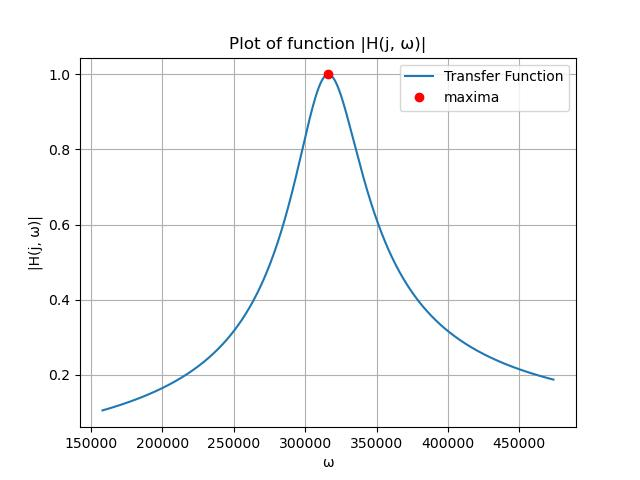
\includegraphics[width=1.0\columnwidth]{2022/IN/33/figs/fig_1.jpg}
    \caption{Transfer function $\abs{H\brak{j, \omega}}$ taken from python3}
    \label{fig:enter-label}
\end{figure}

\pagebreak

\item In the circuit shown below, the switch S is closed at $t=0$. The magnitude of the steady state voltage, in volts, across the $6\Omega$ resistor is \_\_\_\_\_.(\textit{round off to two decimal places})\\ \hfill(GATE 2022 EE Q31)
\begin{figure}[!h]
    \centering
    \begin{circuitikz}[scale = 0.8]
        \draw(0, 0) -- (1, 0);
        \draw(1, 0.5) -- (1, -0.5);
        \draw(4, 0.5) -- (4, -0.5);
        \draw(4, 0) -- (5, 0);

        \draw(1, 0.5) to[R, l = $6\Omega$](4, 0.5);
        \draw(1, -0.5) to[R, l_ = $3\Omega$](4, -0.5);

        \draw(0, 0) -- (0, -2);
        \draw(5, 0) -- (5, -2);

        \draw(0, -2) to[C, l = $1\mu F$](2, -2);
        \draw(2, -2) to [R, l = $10\Omega$](5, -2);

        \draw(0, -2) -- (0, -3.5);
        \draw(5, -2) -- (5, -3.5);

        \draw(0, -3.5) to[battery2, l_ = $10V$](1.5, -3.5);
        \draw (1.5, -3.5) to[switch, l = S] (2, -3.5);
        \draw(2, -3.5) to [R, l = $2\Omega$](5, -3.5);

        \draw[->](0, -3.5) -- (0, -2.5) node[midway, left] {$I$}; 
    \end{circuitikz}
    \caption{}
    \label{fig:1_gate.ee.22.31}
\end{figure}\\
\solution
\iffalse
\let\negmedspace\undefined
\let\negthickspace\undefined
\documentclass[journal,12pt,twocolumn]{IEEEtran}
\usepackage{cite}
\usepackage{amsmath,amssymb,amsfonts,amsthm}
\usepackage{algorithmic}
\usepackage{graphicx}
\usepackage{textcomp}
\usepackage{xcolor}
\usepackage{txfonts}
\usepackage{listings}
\usepackage{enumitem}
\usepackage{mathtools}
\usepackage{gensymb}
\usepackage{comment}
\usepackage[breaklinks=true]{hyperref}
\usepackage{tkz-euclide} 
\usepackage{listings}
\usepackage{gvv}                            \usepackage{tikz}
\usepackage{circuitikz}
\def\inputGnumericTable{}                                
\usepackage[latin1]{inputenc}                            
\usepackage{color}                                       
\usepackage{array}                                       
\usepackage{longtable}                                   
\usepackage{calc}                              
\usepackage{tikz}
\usepackage{multirow}                                    
\usepackage{hhline}                                      
\usepackage{ifthen}                            
\usepackage{caption}
\usepackage{lscape}
\usepackage{amsmath}
\newtheorem{theorem}{Theorem}[section]
\newtheorem{problem}{Problem}
\newtheorem{proposition}{Proposition}[section]
\newtheorem{lemma}{Lemma}[section]
\newtheorem{corollary}[theorem]{Corollary}
\newtheorem{example}{Example}[section]
\newtheorem{definition}[problem]{Definition}
\newcommand{\BEQA}{\begin{eqnarray}}
\newcommand{\EEQA}{\end{eqnarray}}
\newcommand{\define}{\stackrel{\triangle}{=}}
\theoremstyle{remark}
\newtheorem{rem}{Remark}

\begin{document}

\bibliographystyle{IEEEtran}
\vspace{3cm}

\title{GATE 2023 PH Q37}
\author{EE23BTECH11009 - AROSHISH PRADHAN$^{*}$% <-this % stops a space
}
\maketitle
\newpage
\bigskip
\textbf{Question:} In the circuit shown below, the switch S is closed at $t=0$. The magnitude of the steady state voltage, in volts, across the $6\Omega$ resistor is \_\_\_\_\_.(\textit{round off to two decimal places})\\ \hfill(GATE 2022 EE Q31)
\begin{figure}[!h]
    \centering
    \begin{circuitikz}[scale = 0.8]
        \draw(0, 0) -- (1, 0);
        \draw(1, 0.5) -- (1, -0.5);
        \draw(4, 0.5) -- (4, -0.5);
        \draw(4, 0) -- (5, 0);

        \draw(1, 0.5) to[R, l = $6\Omega$](4, 0.5);
        \draw(1, -0.5) to[R, l_ = $3\Omega$](4, -0.5);

        \draw(0, 0) -- (0, -2);
        \draw(5, 0) -- (5, -2);

        \draw(0, -2) to[C, l = $1\mu F$](2, -2);
        \draw(2, -2) to [R, l = $10\Omega$](5, -2);

        \draw(0, -2) -- (0, -3.5);
        \draw(5, -2) -- (5, -3.5);

        \draw(0, -3.5) to[battery2, l_ = $10V$](1.5, -3.5);
        \draw (1.5, -3.5) to[switch, l = S] (2, -3.5);
        \draw(2, -3.5) to [R, l = $2\Omega$](5, -3.5);

        \draw[->](0, -3.5) -- (0, -2.5) node[midway, left] {$I$}; 
    \end{circuitikz}
    \caption{}
    \label{fig:1_gate.ee.22.31}
\end{figure}\\

\solution 
\fi
Consider a sinusoidal input source of angular frequency $\omega$.

\begin{table}[!h]
    \centering
    \begin{tabular}{|c|c|c|}
    \hline
       \textbf{Symbol}  &  \textbf{Value}  &  \textbf{Description}\\
    \hline
       $\omega$  &  $0$ for D.C. &  Angular Frequency\\
    \hline
        $C$ & $1\mu F$ & Capacitance \\
    \hline
        $V_{in}(t)$ & $10\cos(\omega t)$ & Input Voltage\\
    \hline
        $V_{out}(t)$ &  & Output Voltage across $6\Omega$\\
    \hline
        $V_{out}(j\omega)$ & $H(j\omega)V_{in}(j\omega)$ & Output in Frequency Domain\\
    \hline
        $H(j\omega)$ &  & Transfer Function\\
    \hline
        $I(j\omega)$ & & Total Current\\
    \hline
        $Z_{\text{eff}}$ & & Overall Impedance\\
    \hline
    \end{tabular}
    \caption{Given Parameters}
    \label{tab:1_gate.22.ee.31}
\end{table}

Using KCL and KVL, we can calculate:
\begin{align}
    Z_{\text{eff}} &= \frac{2\brak{10 + \frac{1}{j\omega C}}}{12 + \frac{1}{j\omega C}} + 2\\
    \implies I(j\omega) &= \frac{V_{in}}{\brak{\frac{2\brak{10 + \frac{1}{j\omega C}}}{12 + \frac{1}{j \omega C}}+2}}\\
    \implies V_{out}(j\omega) &= 2\sbrak{\brak{\frac{10 + \frac{1}{j\omega C}}{12 + \frac{1}{j\omega C}}}I(j\omega)}\\
    &= 2\sbrak{\brak{\frac{10 + \frac{1}{j\omega C}}{12 + \frac{1}{j\omega C}}}\frac{V_{in}(j\omega)}{\brak{\frac{2\brak{10 + \frac{1}{j\omega C}}}{12 + \frac{1}{j \omega C}}+2}}}\\
    \implies H(j\omega) &= \frac{1 + 10j\omega C}{2(1 + 11j\omega C)}
\end{align}
\begin{figure}[!h]
    \centering
    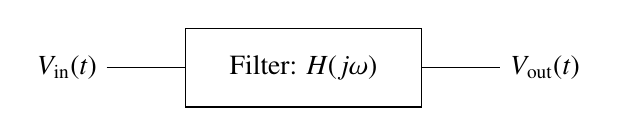
\begin{tikzpicture}
    % Draw the filter rectangle
    \draw (0,0) rectangle (3,1) node[midway] {Filter: $H(j\omega)$};
    
    % Draw the input and output labels
    \draw (-1,0.5) node[left] {$V_{\text{in}}(t)$} -- (0,0.5);
    \draw (3,0.5) -- (4,0.5) node[right] {$V_{\text{out}}(t)$};
\end{tikzpicture}
    \caption{Filter Equivalent of Circuit}
    \label{fig:2_gate.22.ee.31}
\end{figure}
\begin{align}
    H(j\omega) &= \brak{\frac{\sqrt{1 + 100\omega^2 C^2}}{2\sqrt{1 + 121\omega^2 C^2}}}e^{j(\tan^{-1}(10\omega C) - \tan^{-1}(11\omega C))}\\
    &= \brak{\frac{\sqrt{1 + 100\omega^2 C^2}}{2\sqrt{1 + 121\omega^2 C^2}}}e^{j\tan^{-1}\brak{\frac{-\omega C}{1 + 110\omega^2 C^2}}}\\
    \therefore V_{out}(t) &= 10\abs{H(j\omega)}\cos(\omega t + \angle H(j\omega))\\
    &= \frac{5\sqrt{1 + 100\omega^2 C^2}}{\sqrt{1 + 121\omega^2 C^2}}\cos\brak{\omega t -\tan^{-1}\brak{\frac{\omega C}{1 + 110\omega^2 C^2}}}
\end{align}
\begin{figure}[!h]
    \centering
    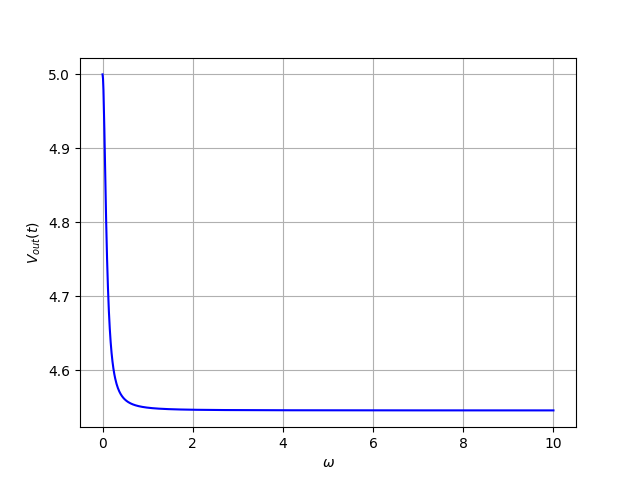
\includegraphics[width = \columnwidth]{2022/EE/31/figs/V_out_plot.png}
    \caption{Plot of $V_{out}(t)$ at $t=0$ w.r.t $\omega$}
    \label{fig:3_gate.22.ee.31}
\end{figure}

As $\omega \rightarrow 0$, $V_{in}(t)$ approaches being a D.C. input source ($10V$).

$\therefore$ substituting $\omega = 0$, we get:
\begin{align}
    V_{out}(t) &= 5V
\end{align}

%\end{document}


\pagebreak

\item An ideal OPAMP circuit with a sinusoidal input is shown in the figure. The 3dB frequency is the frequency at which the magnitude of the voltage gain decreases by 3 dB from the maximum value. Which of the options is/are correct?

\begin{figure}[H]
  \centering
  \begin{circuitikz}

\ctikzset{bipoles/length=1cm}                           
\draw (0, 0) node[op amp] (opamp) {};
\draw (opamp.-) to[R,l_= $1k\Omega$,-] (-2.5, 0.35) -- (-2.7, 0.35) to[C,l_=$1\mu F$,-](-3.35,0.35)  (-3.25,-0.5) node[ground]{};                                 
\draw (opamp.-) to[short,*-] ++(0,0.5) coordinate (leftC) to[R= $2k\Omega$] (leftC -| opamp.out)to[short,-*] (opamp.out) to [short,-*] (1.5,0) (1.5,-0.5) node[ground]{};
\draw (opamp.+) -- (-1,-0.35) to (-1,-0.5) node[ground]{}
;
\draw[thick] (opamp.up) -- +(0,0.2) node[right] {\scriptsize$+15V$};
\draw[thick] (opamp.down) -- +(0,-0.2) node[right] {\scriptsize$-15V$};

% Double-sided arrows for input and output voltage
%\draw[thick,postaction={decorate,decoration={markings,mark=at position 1.0 with {\arrow{stealth}}}}] (-3.35,-0.5) -- (-3.35,0.30) node[midway,left] {$V_{in}$};
%\draw[postaction={decorate,decoration={markings,mark=at position 1.0 with {\arrow{stealth}}}}] (-3.35,0.30) -- (-3.35,-0.5){};
%\draw[thick,postaction={decorate,decoration={markings,mark=at position 1.0 with {\arrow{stealth}}}}] (1.6,0) -- (1.6,-0.7) node[midway,right] {$V_{out}$};
%\draw[postaction={decorate,decoration={markings,mark=at position 1.0 with {\arrow{stealth}}}}] (1.6,-0.7) -- (1.6,0) {};
 
 
\draw[thick, postaction={decorate,decoration={markings,mark=at position 0 with {\node[left] {\scriptsize$-$}; \draw[-latex](0.2,0)--(0,0);},mark=at position 1 with {\node[left] {\scriptsize$+$}; \draw[-latex] (0,0)--(0.2,0);}}}] (-3.35,-0.7) -- (-3.35,0.1) node[midway,left] {\scriptsize$V_{in}$};
\draw[thick, postaction={decorate,decoration={markings,mark=at position 0 with {\node[right] {\scriptsize$+$}; \draw[-latex] (0.2,0)--(0,0);},mark=at position 1 with {\node[right] {\scriptsize$-$}; \draw[-latex] (0,0)--(0.3,0);}}}] (1.6,0) -- (1.6,-0.5) node[midway,right] {\scriptsize$V_{out}$};
                                                          \end{circuitikz}                                        


  \label{fig:26fig1}
\end{figure}

\begin{enumerate}[label=(\Alph*)]
\item The circuit is a low pass filter.\\
\item The circuit is a high pass filter.\\
\item The 3 dB frequency is 1000rad/s.\\
\item The 3 dB frequency is $\frac{1000}{3}$rad/s.\\
\end{enumerate}
\hfill(GATE EC 2022)\\
\solution
\iffalse
\let\negmedspace\undefined
\let\negthickspace\undefined
\documentclass[journal,12pt,twocolumn]{IEEEtran}
\usepackage{cite}
\usepackage{amsmath,amssymb,amsfonts,amsthm}
\usepackage{algorithmic}
\usepackage{graphicx}
\usepackage{textcomp}
\usepackage{xcolor}
\usepackage{txfonts}
\usepackage{listings}
\usepackage{enumitem}
\usepackage{mathtools}
\usepackage{gensymb}
\usepackage{comment}
\usepackage[breaklinks=true]{hyperref}
\usepackage{tkz-euclide} % loads  TikZ and tkz-base
\usepackage{listings}
\usepackage[latin1]{inputenc}                                
\usepackage{color}                                            
\usepackage{array}                                            
\usepackage{longtable}                                       
\usepackage{calc}                                             
\usepackage{multirow}                                         
\usepackage{hhline}                                           
\usepackage{ifthen}                                           
\usepackage{lscape}
\usepackage{caption}
\usepackage{subcaption}
\usepackage{float}
\usepackage{circuitikz}
\usetikzlibrary{decorations.markings} 


\newtheorem{theorem}{Theorem}[section]
\newtheorem{problem}{Problem}
\newtheorem{proposition}{Proposition}[section]
\newtheorem{lemma}{Lemma}[section]
\newtheorem{corollary}[theorem]{Corollary}
\newtheorem{example}{Example}[section]
\newtheorem{definition}[problem]{Definition}
%\newtheorem{thm}{Theorem}[section] 
%\newtheorem{defn}[thm]{Definition}
%\newtheorem{algorithm}{Algorithm}[section]
%\newtheorem{cor}{Corollary}
\newcommand{\BEQA}{\begin{eqnarray}}
\newcommand{\EEQA}{\end{eqnarray}}
\newcommand{\define}{\stackrel{\triangle}{=}}
\theoremstyle{remark}
\newtheorem{rem}{Remark}
%\bibliographystyle{ieeetr}

\begin{document}

%
\providecommand{\pr}[1]{\ensuremath{\Pr\left(#1\right)}}
\providecommand{\prt}[2]{\ensuremath{p_{#1}^{\left(#2\right)} }}        % own macro for this question
\providecommand{\qfunc}[1]{\ensuremath{Q\left(#1\right)}}
\providecommand{\sbrak}[1]{\ensuremath{{}\left[#1\right]}}
\providecommand{\lsbrak}[1]{\ensuremath{{}\left[#1\right.}}
\providecommand{\rsbrak}[1]{\ensuremath{{}\left.#1\right]}}
\providecommand{\brak}[1]{\ensuremath{\left(#1\right)}}
\providecommand{\lbrak}[1]{\ensuremath{\left(#1\right.}}
\providecommand{\rbrak}[1]{\ensuremath{\left.#1\right)}}
\providecommand{\cbrak}[1]{\ensuremath{\left\{#1\right\}}}
\providecommand{\lcbrak}[1]{\ensuremath{\left\{#1\right.}}
\providecommand{\rcbrak}[1]{\ensuremath{\left.#1\right\}}}
\newcommand{\sgn}{\mathop{\mathrm{sgn}}}
\providecommand{\abs}[1]{\left\vert#1\right\vert}
\providecommand{\res}[1]{\Res\displaylimits_{#1}} 
\providecommand{\norm}[1]{\left\lVert#1\right\rVert}
%\providecommand{\norm}[1]{\lVert#1\rVert}
\providecommand{\mtx}[1]{\mathbf{#1}}
\providecommand{\mean}[1]{E\left[ #1 \right]}
\providecommand{\cond}[2]{#1\middle|#2}
\providecommand{\fourier}{\overset{\mathcal{F}}{ \rightleftharpoons}}
\newenvironment{amatrix}[1]{%
  \left(\begin{array}{@{}*{#1}{c}|c@{}}
}{%
  \end{array}\right)
}
%\providecommand{\hilbert}{\overset{\mathcal{H}}{ \rightleftharpoons}}
%\providecommand{\system}{\overset{\mathcal{H}}{ \longleftrightarrow}}
        %\newcommand{\solution}[2]{\textbf{Solution:}{#1}}
\newcommand{\solution}{\noindent \textbf{Solution: }}
\newcommand{\cosec}{\,\text{cosec}\,}
\providecommand{\dec}[2]{\ensuremath{\overset{#1}{\underset{#2}{\gtrless}}}}
\newcommand{\myvec}[1]{\ensuremath{\begin{pmatrix}#1\end{pmatrix}}}
\newcommand{\mydet}[1]{\ensuremath{\begin{vmatrix}#1\end{vmatrix}}}
\newcommand{\myaugvec}[2]{\ensuremath{\begin{amatrix}{#1}#2\end{amatrix}}}
\providecommand{\rank}{\text{rank}}
\providecommand{\pr}[1]{\ensuremath{\Pr\left(#1\right)}}
\providecommand{\qfunc}[1]{\ensuremath{Q\left(#1\right)}}
        \newcommand*{\permcomb}[4][0mu]{{{}^{#3}\mkern#1#2_{#4}}}
\newcommand*{\perm}[1][-3mu]{\permcomb[#1]{P}}
\newcommand*{\comb}[1][-1mu]{\permcomb[#1]{C}}
\providecommand{\qfunc}[1]{\ensuremath{Q\left(#1\right)}}
\providecommand{\gauss}[2]{\mathcal{N}\ensuremath{\left(#1,#2\right)}}
\providecommand{\diff}[2]{\ensuremath{\frac{d{#1}}{d{#2}}}}
\providecommand{\myceil}[1]{\left \lceil #1 \right \rceil }
\newcommand\figref{Fig.~\ref}
\newcommand\tabref{Table~\ref}
\newcommand{\sinc}{\,\text{sinc}\,}
\newcommand{\rect}{\,\text{rect}\,}
%%
%       %\newcommand{\solution}[2]{\textbf{Solution:}{#1}}
%\newcommand{\solution}{\noindent \textbf{Solution: }}
%\newcommand{\cosec}{\,\text{cosec}\,}
%\numberwithin{equation}{section}
%\numberwithin{equation}{subsection}
%\numberwithin{problem}{section}
%\numberwithin{definition}{section}
%\makeatletter
%\@addtoreset{figure}{problem}
%\makeatother

%\let\StandardTheFigure\thefigure
\let\vec\mathbf

\bibliographystyle{IEEEtran}

\vspace{3cm}
\title{Assignment}
\author{EE23BTECH11001 - Aashna Sahu}
\maketitle
\bigskip

\renewcommand{\thefigure}{\theenumi}
\renewcommand{\thetable}{\theenumi}
%\renewcommand{\theequation}{\theenumi}

Q:An ideal OPAMP circuit with a sinusoidal input is shown in the figure. The 3dB frequency is the frequency at which the magnitude of the voltage gain decreases by 3 dB from the maximum value. Which of the options is/are correct?

\begin{figure}[H]
  \centering
  \begin{circuitikz}

\ctikzset{bipoles/length=1cm}                           
\draw (0, 0) node[op amp] (opamp) {};
\draw (opamp.-) to[R,l_= $1k\Omega$,-] (-2.5, 0.35) -- (-2.7, 0.35) to[C,l_=$1\mu F$,-](-3.35,0.35)  (-3.25,-0.5) node[ground]{};                                 
\draw (opamp.-) to[short,*-] ++(0,0.5) coordinate (leftC) to[R= $2k\Omega$] (leftC -| opamp.out)to[short,-*] (opamp.out) to [short,-*] (1.5,0) (1.5,-0.5) node[ground]{};
\draw (opamp.+) -- (-1,-0.35) to (-1,-0.5) node[ground]{}
;
\draw[thick] (opamp.up) -- +(0,0.2) node[right] {\scriptsize$+15V$};
\draw[thick] (opamp.down) -- +(0,-0.2) node[right] {\scriptsize$-15V$};

% Double-sided arrows for input and output voltage
%\draw[thick,postaction={decorate,decoration={markings,mark=at position 1.0 with {\arrow{stealth}}}}] (-3.35,-0.5) -- (-3.35,0.30) node[midway,left] {$V_{in}$};
%\draw[postaction={decorate,decoration={markings,mark=at position 1.0 with {\arrow{stealth}}}}] (-3.35,0.30) -- (-3.35,-0.5){};
%\draw[thick,postaction={decorate,decoration={markings,mark=at position 1.0 with {\arrow{stealth}}}}] (1.6,0) -- (1.6,-0.7) node[midway,right] {$V_{out}$};
%\draw[postaction={decorate,decoration={markings,mark=at position 1.0 with {\arrow{stealth}}}}] (1.6,-0.7) -- (1.6,0) {};
 
 
\draw[thick, postaction={decorate,decoration={markings,mark=at position 0 with {\node[left] {\scriptsize$-$}; \draw[-latex](0.2,0)--(0,0);},mark=at position 1 with {\node[left] {\scriptsize$+$}; \draw[-latex] (0,0)--(0.2,0);}}}] (-3.35,-0.7) -- (-3.35,0.1) node[midway,left] {\scriptsize$V_{in}$};
\draw[thick, postaction={decorate,decoration={markings,mark=at position 0 with {\node[right] {\scriptsize$+$}; \draw[-latex] (0.2,0)--(0,0);},mark=at position 1 with {\node[right] {\scriptsize$-$}; \draw[-latex] (0,0)--(0.3,0);}}}] (1.6,0) -- (1.6,-0.5) node[midway,right] {\scriptsize$V_{out}$};
                                                          \end{circuitikz}                                        


  \label{fig:26fig1}
\end{figure}



\begin{enumerate}[label=(\Alph*)]
\item The circuit is a low pass filter.\\
\item The circuit is a high pass filter.\\
\item The 3 dB frequency is 1000rad/s.\\
\item The 3 dB frequency is $\frac{1000}{3}$rad/s.\\
\end{enumerate}
\hfill(GATE EC 2022)

\solution
\fi
\begin{table}[ht]
  \centering
  \begin{tabular}{|c|c|c|}
      \hline
      Parameter & Description & Value\\\hline
      $V_{in}$ & Input Voltage & --\\\hline
      $V_{out}$ & Output Voltage & --\\\hline
      $C$ & Capacitor & $1\mu F$\\\hline
      $R_1$ & Resistance & $1k\Omega$\\\hline
      $R_2$ & Feedback Resistance & $2k\Omega$\\\hline
      $V$ & Voltage at Negative terminal & --\\\hline
      $V^+$ & Voltage at positive terminal & 0\\\hline
\end{tabular}

  \caption{Input Parameters}
  \label{tab:26tab1}
\end{table}

\begin{figure}[H]
  \centering
  \begin{circuitikz}                                                                            

\ctikzset{bipoles/length=1cm}                           
\draw (0, 0) node[op amp] (opamp) {};
\draw (opamp.-) to[R,l_= $1k\Omega$,-,i<_=\scriptsize$I$] (-2.5, 0.35) -- (-2.7, 0.35) to[C,l_=$1\mu F$,-](-3.35,0.35)  (-3.25,-0.5) node[ground]{};                                 
\draw (opamp.-) to[short,*-] ++(0,0.5) coordinate (leftC) to[R= $2k\Omega$,i>^=\scriptsize$I$] (leftC -| opamp.out)to[short,-*] (opamp.out) to [short,-*] (1.5,0) (1.5,-0.5) node[ground]{};
\draw (opamp.+) -- (-1,-0.35) to (-1,-0.5) node[ground]{}
;
\draw[thick] (opamp.up) -- +(0,0.2) node[right] {\scriptsize$+15V$};
\draw[thick] (opamp.down) -- +(0,-0.2) node[right] {\scriptsize$-15V$};

% Double-sided arrows for input and output voltage
%\draw[thick,postaction={decorate,decoration={markings,mark=at position 1.0 with {\arrow{stealth}}}}] (-3.35,-0.5) -- (-3.35,0.30) node[midway,left] {$V_{in}$};
%\draw[postaction={decorate,decoration={markings,mark=at position 1.0 with {\arrow{stealth}}}}] (-3.35,0.30) -- (-3.35,-0.5){};
%\draw[thick,postaction={decorate,decoration={markings,mark=at position 1.0 with {\arrow{stealth}}}}] (1.6,0) -- (1.6,-0.7) node[midway,right] {$V_{out}$};
%\draw[postaction={decorate,decoration={markings,mark=at position 1.0 with {\arrow{stealth}}}}] (1.6,-0.7) -- (1.6,0) {};
 
 
\draw[thick, postaction={decorate,decoration={markings,mark=at position 0 with {\node[left] {\scriptsize$-$}; \draw[-latex](0.2,0)--(0,0);},mark=at position 1 with {\node[left] {\scriptsize$+$}; \draw[-latex] (0,0)--(0.2,0);}}}] (-3.35,-0.7) -- (-3.35,0.1) node[midway,left] {\scriptsize$V_{in}$};
\draw[thick, postaction={decorate,decoration={markings,mark=at position 0 with {\node[right] {\scriptsize$+$}; \draw[-latex] (0.2,0)--(0,0);},mark=at position 1 with {\node[right] {\scriptsize$-$}; \draw[-latex] (0,0)--(0.3,0);}}}] (1.6,0) -- (1.6,-0.5) node[midway,right] {\scriptsize$V_{out}$};
\node at (-0.78, 0.15) {\scriptsize$V$}; 
                                        
\end{circuitikz} 
                                                                         


  \label{fig:26fig2}
\end{figure}

\begin{align}
\frac{V_{in}-V}{\frac{1}{sC}+R_1}=\frac{V-V_{out}}{R_2}
\end{align}
As Op-Amp is ideal
\begin{align}
V=V^+=0V\\
\abs{\frac{V_{out}}{V_{in}}}=\frac{sCR_2}{1+sCR_1}\\
H(s)=\frac{sCR_2}{1+sCR_1}
\label{eq:26eq4}
\end{align}
Keeping $s=j\omega$\\
For determining nature of Filter\\
Put $j\omega=0$
\begin{align}
H(j\omega)=0
\end{align}
Put $j\omega\rightarrow \infty$
\begin{align}
H(j\omega)=\frac{R_2}{R_1}=2\quad (\text{Finite})
\end{align}\\
$\therefore$ It is high pass filter.\\

On simplifying \eqref{eq:26eq4} further
\begin{align}
H(j\omega)=\frac{R_2}{R_1}\left(\frac{j\omega}{j\omega+\frac{1}{CR_1}}\right)\\
\abs{H(j\omega)}_{max}=\frac{R_2}{R_1} \label{eq:26eq8}\\
\abs{H(j\omega)}_{\omega=\omega_c}=\frac{R_2}{R_1}\abs{\frac{j\omega_c}{j\omega_c+\frac{1}{CR_1}}}
\label{eq:26eq9}
\end{align}
%\textbf{Alternate}\\
%Generally for first order transfer function

%\begin{align}
%H(s)|_{LPF}=\frac{1}{s+\omega}\\
%H(s)|_{HPF}=\frac{s}{s+\omega}
%\label{eq:eq8}
%\end{align}
Given: 
\begin{align}
20\log(\abs{H(j\omega)}_{max})-20\log(\abs{H(j\omega)}_{\omega=\omega_c})=3 dB
\end{align}
\begin{align}
\frac{\abs{H(j\omega)}_{max}}{\abs{H(j\omega)}_{\omega=\omega_c}}=\sqrt 2
\end{align}
 
From \eqref{eq:26eq8} and \eqref{eq:26eq9}
\begin{align}
\frac{R_2}{R_1}\abs{\frac{j\omega_c}{j\omega_c+\frac{1}{CR_1}}}&=\frac{1}{\sqrt 2}\frac{R_2}{R_1}\\
\abs{\frac{j\omega_c}{j\omega_c+\frac{1}{CR_1}}}&=\frac{1}{\sqrt 2}\\
\implies \omega_c &= \frac{1}{CR_1}
\end{align}
From \tabref{tab:26tab1}
\begin{align}
\omega_c= 1000 \text{rad/s}
\end{align}
Where $\omega_c$ is 3 dB frequency.\\

Finally, Correct options are (B) and (C).

\begin{figure}[H]
  \centering
  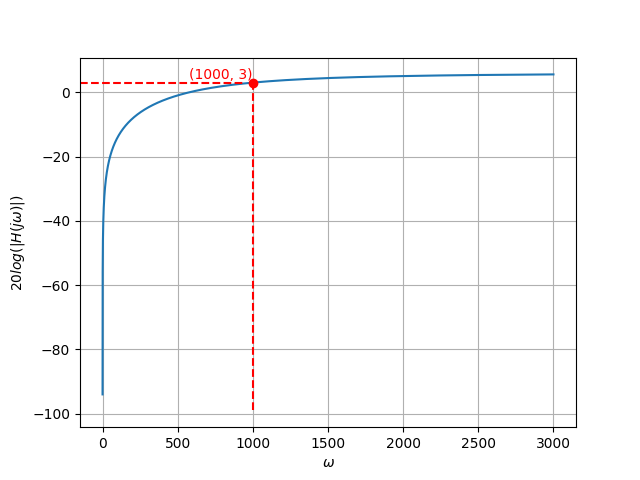
\includegraphics[width=1.0\columnwidth]{2022/EC/26/figs/plot1.png}
  \caption{\centering Frequency response plot}
  \label{fig:26fig3}
\end{figure}
%\end{document}



\pagebreak

\item A series $RLC$ circuit with $R = 10 \Omega$, $L = 50 mH$ and $C = 100 \micro F$ connected to
$200$ $V$, $50$ Hz supply consumes power $P$. The value of $L$ is changed such that this
circuit consumes same power $P$ but operates with lagging power factor. The new
value of L is $\hrulefill$ $mH$ (rounded off to two decimal places).
\hfill(GATE 33 BM 2022)

\solution
\iffalse
\let\negmedspace\undefined
\let\negthickspace\undefined
\documentclass[journal,12pt,twocolumn]{IEEEtran}
\usepackage{cite}
\usepackage{amsmath,amssymb,amsfonts,amsthm}
\usepackage{algorithmic}
\usepackage{graphicx}
\usepackage{textcomp}
\usepackage{xcolor}
\usepackage{txfonts}
\usepackage{listings}
\usepackage{enumitem}
\usepackage{mathtools}
\usepackage{gensymb}
\usepackage{comment}
\usepackage[breaklinks=true]{hyperref}
\usepackage{tkz-euclide} 
\usepackage{tikz}
\usepackage{circuitikz}
\usepackage{listings}
\usepackage{gvv}                                        
\def\inputGnumericTable{}                                 
\usepackage[latin1]{inputenc}                                
\usepackage{color}                                            
\usepackage{array}                                            
\usepackage{longtable}                                       
\usepackage{calc}                                             
\usepackage{multirow}                                         
\usepackage{hhline}                                           
\usepackage{ifthen}                                           
\usepackage{lscape}
\usepackage{caption}
\newtheorem{theorem}{Theorem}[section]
\newtheorem{problem}{Problem}
\newtheorem{proposition}{Proposition}[section]
\newtheorem{lemma}{Lemma}[section]
\newtheorem{corollary}[theorem]{Corollary}
\newtheorem{example}{Example}[section]
\newtheorem{definition}[problem]{Definition}
\newcommand{\BEQA}{\begin{eqnarray}}
\newcommand{\EEQA}{\end{eqnarray}}
\newcommand{\define}{\stackrel{\triangle}{=}}
\theoremstyle{remark}
\newtheorem{rem}{Remark}
\begin{document}
\parindent 0px
\bibliographystyle{IEEEtran}
\vspace{3cm}

\title{GATE 2022 33.BM}
\author{EE23BTECH11012 - Chavan Dinesh$^{*}$% <-this % stops a space
}
\maketitle
\newpage
\bigskip

\renewcommand{\thefigure}{\arabic{figure}}
\renewcommand{\thetable}{\arabic{table}}
\large\textbf{\textsl{Question:}}
A series $RLC$ circuit with $R = 10 \Omega$, $L = 50 mH$ and $C = 100 \micro F$ connected to
$200$ $V$, $50$ Hz supply consumes power $P$. The value of $L$ is changed such that this
circuit consumes same power $P$ but operates with lagging power factor. The new
value of L is $\hrulefill$ $mH$ (rounded off to two decimal places).
\hfill(GATE 33 BM 2022)

\solution
\fi
\begin{table}[htbp]
    \centering
    \begin{tabular}{|c|c|c|}
\hline
   \textbf{Parameter}  & \textbf{Description} & \textbf{Value}\\
   \hline
   $R$   & Resistance & $10 \Omega$\\
   \hline
  $C$ & Capacitance & $100 \micro F$ \\
  \hline
  $L_{old}$ & Inductor & $50mH$\\
  \hline
  $L_{new}$ & New Inductor &    \\
  \hline
  $Z_{old}$ & Old Impedance & \\
  \hline
  $Z^*$ &New Impedance & \\
  \hline
  
\end{tabular}

    \caption{}
    \label{tab:input_parameters.33.BM.2022}
\end{table}

\begin{figure}[!ht]
    \centering
        \begin{circuitikz}
    \draw(0, 0) -- (1, 0);
    \draw(1, 0) to [L, l = $50\text{mH}$](2, 0);
    \draw(2, 0) -- (3, 0);
    \draw(3, 0) to [C, l = $100\, \mu\text{F}$](4, 0);
    \draw(4, 0) -- (5, 0);
    \draw(5, 0) to [R, l = $10\Omega$](6, 0);
    \draw(0, 0) -- (0, -2);
    \draw[->] (0, -1) node[left] {$I(t)$} -- (0, -1);
    \draw(6, 0) -- (7, 0);
    \draw(7, 0) -- (7, -2);
    \draw(0, -2) -- (3, -2);
    \draw(7, -2) -- (7, -2);
    \draw(3, -2) to [sV, l = $V(t)$](4, -2);
    \draw(4, -2) -- (7, -2);
\end{circuitikz}

    \caption{}
    \label{fig:fig1.33.BM.2022}
\end{figure}

From \figref{fig:fig1.33.BM.2022}

In $s$ - domain,
\begin{figure}[htbp]
    \centering
    \begin{circuitikz}
    \draw(0, 0) -- (1, 0);
    \draw(1, 0) to [L, l = $sL$](2, 0);
    \draw(2, 0) -- (3, 0);
    \draw(3, 0) to [C, l = $\frac{1}{sC}$](4, 0);
    \draw(4, 0) -- (5, 0);
    \draw(5, 0) to [R, l = $R$](6, 0);
    \draw(0, 0) -- (0, -2);
    \draw[->] (0, -1) node[left] {$I(s)$} -- (0, -1);
    \draw(6, 0) -- (7, 0);
    \draw(7, 0) -- (7, -2);
    \draw(0, -2) -- (3, -2);
    \draw(7, -2) -- (7, -2);
    \draw(3, -2) to [sV, l = $V(s)$](4, -2);
    \draw(4, -2) -- (7, -2);
\end{circuitikz}

\end{figure}

  \begin{align}
      Z = R + sL_{old} + \frac{1}{sC}
  \end{align}
As the circuit consumes same power $P$ but operates with lagging power factor : 

The new impedance($Z^*$) will be :
\begin{align}
    Z^* =  R + sL_{new} + \frac{1}{sC}
\end{align}
Comparing the imaginary parts of the impedances:
\begin{align}
    sL_{old} + \frac{1}{sC} = -\left( sL_{new} + \frac{1}{sC}\right)
    \end{align}
Taking $s = j2\pi f$ :
\begin{align}
     j\left(2\pi fL_{old} - \frac{1}{2\pi fC}\right)  =  -j\left(2\pi fL_{new} - \frac{1}{2\pi fC}\right)
\end{align}
From \tabref{tab:input_parameters.33.BM.2022}:
\begin{align}
    L_{new} \approx 152.7 \text{mH}
\end{align}

% \begin{figure}[ht]
%     \centering
%     \includegraphics[width = \columnwidth]{figs/x_n_stem_plot.png}
%     \caption{}
%     \label{fig:graph1.11.9.3.28}
% \end{figure}



\pagebreak

\item A single-phase full-bridge diode rectifier feeds a resistive load of $50 \Omega$ from a 200 V,
50 Hz single phase AC supply. If the diodes are ideal, then the active power, in watts,
drawn by the load is \rule{1cm}{0.5mm} (round off to nearest integer).  \\
\hfill (GATE EE 32)\\
\solution
\iffalse
\documentclass[journal,12pt,twocolumn]{IEEEtran}
\usepackage{amsmath,amssymb,amsfonts,amsthm}
\usepackage{txfonts}
\usepackage{tkz-euclide}
\usepackage{listings}
\usepackage{gvv}
\usepackage[latin1]{inputenc}
\usepackage{adjustbox}
\usepackage{array}
\usepackage{tabularx}
\usepackage{pgf}
\usepackage{lmodern}
\usepackage{circuitikz}
\usepackage{tikz}
\usepackage{graphicx}
\usepackage[english]{babel}

\begin{document}
\bibliographystyle{IEEEtran}

\vspace{3cm}

\title{}
\author{EE23BTECH11047 - Deepakreddy P
}
\maketitle
\newpage
\bigskip

\noindent \textbf{32} \quad A single-phase full-bridge diode rectifier feeds a resistive load of $50 \Omega$ from a 200 V,
50 Hz single phase AC supply. If the diodes are ideal, then the active power, in watts,
drawn by the load is \rule{1cm}{0.5mm} (round off to nearest integer).  \\
\hfill (GATE EE 32)\\
\solution\\
\fi

\begin{figure}[ht]
  \centering
      \begin{circuitikz}[american]
   \draw (0,8) to [sV=200V](0,-1) to [short](6,-1) to [short](6,0) to [D,l=$D_3$](9,3);
   \draw (0,8) to [short](6,8) to [short](6,6);
   \draw (6,6) to [D,l=$D_1$](9,3);
   \draw (3,3) to [D,l=$D_4$](6,6);
   \draw (3,3) to [D,l=$D_2$](6,0);
   \draw (3,3) to [short](2.5,3) to [crossing, bipoles/crossing/size=1](2.5,-4.8) to [short](12,-4.8) to [R=50$\Omega$](12,3) to [short](9,3);
   \draw (9,3) to [short,i=\Large{I}](12,3);
\end{circuitikz}

  \caption{Circuit-1}
\end{figure}

\begin{figure}[ht]
   \centering
   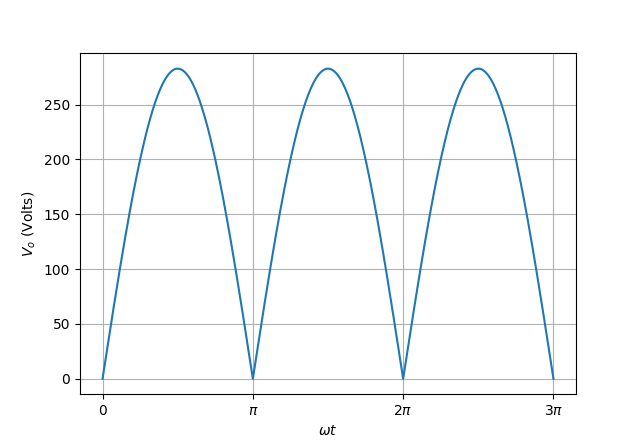
\includegraphics[width=1.2\columnwidth]{2022/EE/32/figs/gt1.png}
   \caption{Output voltage waveform of single-phase full
bridge rectifier}
\end{figure}


\begin{center}
    \begin{table}[ht]
        \setlength{\arrayrulewidth}{0.3mm}
\setlength{\tabcolsep}{12pt}
\renewcommand{\arraystretch}{1.3}


\begin{center}
\caption{Input Parameters}
\begin{tabular}{ |p{1.7cm}|p{1.7cm}|p{1.7cm}|  }

\hline
 {Symbol}&{Description} & {value}\\
\hline
R & Load Resistance & 50$\Omega$\\
\hline
$V_{rms}$ & RMS Voltage  & 200V\\
\hline
f & Frequency & 50Hz \\
\hline

\end{tabular}
\end{center}

    \end{table}
\end{center}

\begin{align}
    V_{rms} &= 200\\
    P &= \frac{\brak{V_{rms}}^2}{R}\\
    P &= \frac{\brak{200}^2}{50}W\\
    P &= 800W
\end{align}


%\end{document}


\pagebreak

\item The circuit shown is driven by a sinusoidal input voltage, $V_{\text{in}}$, resulting in the output voltage $V_{\text{out}}$. The frequency (in kilohertz) at which the voltage gain is 0 dB is (rounded off to two decimal places).
\begin{figure}[htb]
  \centering
  
\begin{circuitikz}
\tikzstyle{every node}=[font=\Large]
\draw [](10,10.5) to[short] (10,12.75);
\draw [](12.5,10.5) to[short] (12.5,12.75);
\draw (10,12.75) to[C] (12.5,12.75);
\draw (10.625,8.5) node[ieeestd buffer port, anchor=in](port){} (port.out) to[short] (12.25,8.5); \draw (port.in) to[short] (10.5,8.5);
\draw [](12.25,8.5) to[short, -o] (14.5,8.5);
\draw [](12.5,10.5) to[short] (12.5,8.5);
\draw [](11.25,9.75) to[short] (11.25,8.75);
\draw [](11.25,8.25) to[short] (11.25,7);
\draw [short] (10.75,8.5) -- (8.5,8.5);
\draw[] (11,8.25) to[short] (10,8.25);
\draw (10,8.25) to (10,7.25) node[ground]{};
\draw [](10,10.5) to[short] (10,8.5);
\draw (7,8.5) to[sinusoidal voltage source, sources/symbol/rotate=auto,l={ \LARGE $Vin$}] (7,6);
\draw (7,6) to (7,5.75) node[ground]{};
\node [font=\Large] at (11,13.5) {1 nF};
\node [font=\Large] at (5.75,7.25) {};
\node [font=\Large] at (15,8) {Vout};
\node [font=\Large] at (11.5,7.25) {-};
\node [font=\Large] at (11.5,9.75) {+};
\draw (10,10.75) to[R,l={ \Large $100k$}] (12.5,10.75);
\draw (7,8.5) to[R,l={ \Large $10k$}] (8.5,8.5);
\end{circuitikz}


\end{figure}
\hfill(GATE IN 2022)\\
\solution
\iffalse
\documentclass[journal,12pt,twocolumn]{IEEEtran}
\usepackage{cite}
\usepackage{amsmath,amssymb,amsfonts,amsthm}
\usepackage{algorithmic}
\usepackage{graphicx}
\usepackage{textcomp}
\usepackage{xcolor}
\usepackage{txfonts}
\usepackage{listings}
\usepackage{enumitem}
\usepackage{mathtools}
\usepackage{gensymb}
\usepackage{comment}
\usepackage[breaklinks=true]{hyperref}
\usepackage{tkz-euclide}
\usepackage{braket}
\def\inputGnumericTable{}
\usepackage[latin1]{inputenc}
\usepackage{color}
\usepackage{array}
\usepackage{longtable}
\usepackage{calc}
\usepackage{multirow}
\usepackage{hhline}
\usepackage{ifthen}
\usepackage{lscape}
\usepackage{gvv} 
\usepackage{circuitikz}

\newtheorem{theorem}{Theorem}[section]
\newtheorem{problem}{Problem}
\newtheorem{proposition}{Proposition}[section]
\newtheorem{lemma}{Lemma}[section]
\newtheorem{corollary}[theorem]{Corollary}
\newtheorem{example}{Example}[section]
\newtheorem{definition}[problem]{Definition}
\newcommand{\BEQA}{\begin{eqnarray}}
\newcommand{\EEQA}{\end{eqnarray}}
\newcommand{\define}{\stackrel{\triangle}{=}}
\theoremstyle{remark}
\newtheorem{rem}{Remark}

\begin{document}

\bibliographystyle{IEEEtran}
\vspace{3cm}

\title{GATE 2022 IN-56}
\author{EE23BTECH11201 - Abburi Tanusha$^{*}$% <-this % stops a space
}
\maketitle
\newpage
\bigskip

\renewcommand{\thefigure}{\theenumi}
\renewcommand{\thetable}{\theenumi}

\vspace{3cm}

\maketitle
\textbf{Question:} 
The circuit shown is driven by a sinusoidal input voltage, $V_{\text{in}}$, resulting in the output voltage $V_{\text{out}}$. The frequency (in kilohertz) at which the voltage gain is 0 dB is (rounded off to two decimal places).
\begin{figure}[htb]
	\centering
	
\begin{circuitikz}
\tikzstyle{every node}=[font=\Large]
\draw [](10,10.5) to[short] (10,12.75);
\draw [](12.5,10.5) to[short] (12.5,12.75);
\draw (10,12.75) to[C] (12.5,12.75);
\draw (10.625,8.5) node[ieeestd buffer port, anchor=in](port){} (port.out) to[short] (12.25,8.5); \draw (port.in) to[short] (10.5,8.5);
\draw [](12.25,8.5) to[short, -o] (14.5,8.5);
\draw [](12.5,10.5) to[short] (12.5,8.5);
\draw [](11.25,9.75) to[short] (11.25,8.75);
\draw [](11.25,8.25) to[short] (11.25,7);
\draw [short] (10.75,8.5) -- (8.5,8.5);
\draw[] (11,8.25) to[short] (10,8.25);
\draw (10,8.25) to (10,7.25) node[ground]{};
\draw [](10,10.5) to[short] (10,8.5);
\draw (7,8.5) to[sinusoidal voltage source, sources/symbol/rotate=auto,l={ \LARGE $Vin$}] (7,6);
\draw (7,6) to (7,5.75) node[ground]{};
\node [font=\Large] at (11,13.5) {1 nF};
\node [font=\Large] at (5.75,7.25) {};
\node [font=\Large] at (15,8) {Vout};
\node [font=\Large] at (11.5,7.25) {-};
\node [font=\Large] at (11.5,9.75) {+};
\draw (10,10.75) to[R,l={ \Large $100k$}] (12.5,10.75);
\draw (7,8.5) to[R,l={ \Large $10k$}] (8.5,8.5);
\end{circuitikz}


\end{figure}
\hfill(GATE IN 2022)\\
\textbf{Solution:} 
\fi

This circuit is an inverting OP-AMP. The transfer function of an inverting OP-AMP is given by\\
\begin{table}[h]
 	\centering
 	\resizebox{14 cm}{!}{
 		
\begin{tabular}{|c|c|c|}
\hline
\textbf{Parameter} &  \textbf{Value} & \textbf{Description} \\
\hline
 $20 \log \brak{\frac{V_{\text{out}}}{V_{\text{in}}}}$ & $0$ &Voltage gain\\
\hline
 Sinusoidal input voltage & $V_{\text{in}}$ & Input voltage applied to the circuit \\
\hline
 Output voltage & $V_{\text{out}}$ & Voltage across the output of the circuit \\
\hline
$R_1$ & 10 k$\Omega$ & Resistor connected to the inverting input of the OP-AMP \\
\hline
$R_2$ & 100 k$\Omega$ & Feedback resistor connected from the output to the inverting input of the OP-AMP \\
\hline
$C$ & 1 nF & Capacitor connected in parallel with $R_2$ \\
 \hline
 $Z_1$ &  ? & Impedance of resistor $R_1$ \\
 \hline
$Z_2$ & ? & Impedance of capacitor $C$ in series with resistor $R_2$ \\
\hline
\end{tabular}



 	}
 	\vspace{6 pt}
 	\caption{Parameters}
 \end{table}
\begin{align}
Z_1 &= R_1 \\
Z_2 &= \frac{R_2}{1+j \omega R_2C} \\
\frac{1}{Z_2} &= \frac{1}{R_2} + j\omega C \\
\frac{V_{\text{out}}}{V_{\text{in}}} &= -\frac{Z_2}{Z_1} \\
\frac{|V_{\text{out}}|}{|V_{\text{in}}|} &= \frac{|Z_2|}{|Z_1|} 
\end{align}
\begin{align}
20 \log \brak{\frac{V_{\text{out}}}{V_{\text{in}}}} &= 0 \\
\frac{V_{\text{out}}}{V_{\text{in}}} &= 1
\end{align}

\begin{align}
\frac{|V_{\text{out}}|}{|V_{\text{in}}|} &= \frac{|R_2|}{|(1+ j\omega R_2C)R_1|} = 1 \\
\frac{R_2}{R_1} &= \sqrt{1 + \brak{R_2 \omega C}^2} \\
10 &= \sqrt{1 + \brak{10^5 \cdot \omega 10^-9}^2} \\
99 &= \omega^2 \times 10^{-8} \\
\omega &= \sqrt{99} \times 10^4 \\
2\pi f &= 99.49 \times 10^3 \\
f &= 15.84 \, \text{kHz}
\end{align}
\begin{figure}[h!]
\centering
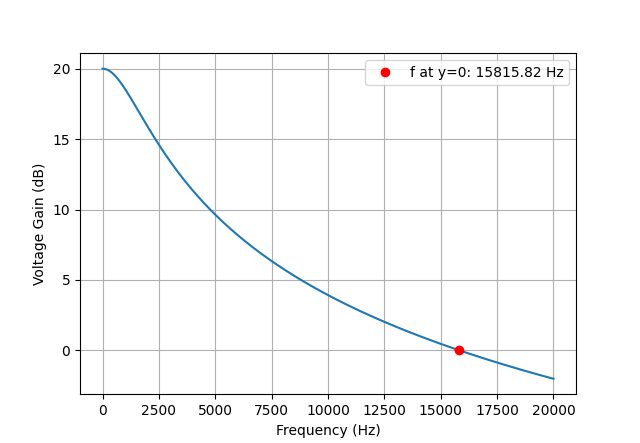
\includegraphics[width=\columnwidth]{2022/IN/56/figs/plot.png}
\caption{Frequency vs Voltage gain}
\end{figure}

%\end{document}


\pagebreak

\item An inductor having a $Q$-factor of 60 is connected in series with a capacitor having a $Q$-factor of 240. The overall $Q$-factor of the circuit is \_\_\_\_\_\_\_\_\_\_. (Round off to the nearest integer) \\
\hfill Gate 2022 EE Question 27\\
\solution
\iffalse
\let\negmedspace\undefined
\let\negthickspace\undefined
\documentclass[journal,12pt,twocolumn]{IEEEtran}
\usepackage{cite}
\usepackage{amsmath,amssymb,amsfonts,amsthm}
\usepackage{algorithmic}
\usepackage{graphicx}
\usepackage{textcomp}
\usepackage{xcolor}
\usepackage{txfonts}
\usepackage{listings}
\usepackage{enumitem}
\usepackage{mathtools}
\usepackage{gensymb}
\usepackage{comment}
\usepackage[breaklinks=true]{hyperref}
\usepackage{tkz-euclide} 
\usepackage{listings}                                   
\def\inputGnumericTable{}                                 
\usepackage[latin1]{inputenc}                                
\usepackage{color}                                            
\usepackage{array}                                            
\usepackage{longtable}                                       
\usepackage{calc}  
\usepackage{circuitikz}                                           
\usepackage{multirow}                                         
\usepackage{hhline}                                           
\usepackage{ifthen}                                           
\usepackage{lscape}
\newtheorem{theorem}{Theorem}[section]
\newtheorem{problem}{Problem}
\newtheorem{proposition}{Proposition}[section]
\newtheorem{lemma}{Lemma}[section]
\newtheorem{corollary}[theorem]{Corollary}
\newtheorem{example}{Example}[section]
\newtheorem{definition}[problem]{Definition}
\newcommand{\BEQA}{\begin{eqnarray}}
\newcommand{\EEQA}{\end{eqnarray}}
\newcommand{\define}{\stackrel{\triangle}{=}}
\newcommand{\brak}[1]{\langle #1 \rangle}
\theoremstyle{remark}
\newtheorem{rem}{Remark}

\begin{document}
\bibliographystyle{IEEEtran}
\vspace{3cm}
\title{\textbf{GATE 2022 EE}}
\author{EE23BTECH11023-ABHIGNYA GOGULA}
\maketitle
\newpage
\bigskip
\renewcommand{\thefigure}{\theenumi}
\renewcommand{\thetable}{\theenumi}
\textbf{Question27:}
\\An inductor having a $Q$-factor of 60 is connected in series with a capacitor having a $Q$-factor of 240. The overall $Q$-factor of the circuit is \_\_\_\_\_\_\_\_\_\_. (Round off to the nearest integer) \\
\hfill Gate 2022 EE Question 27\\
\section*{Solution}
\fi
\begin{circuitikz}
    \draw (0,0) to[R, l=$R_1$] (2,0) to[L, l=$L$] (4,0);
\end{circuitikz}
\begin{align}
Q_1=\frac{\omega_0 L}{R_1}
\end{align}
\begin{circuitikz}
    \draw (0,0) to[R, l=$R_2$] (2,0) to[C, l=$C$] (4,0);
\end{circuitikz}
\begin{align}
Q_2=\frac{1}{\omega_0 C R_2}
\end{align}
at resonance as $\omega_0 L =\frac{1}{\omega_0 C}$ hence
\begin{align}
Q_2=\frac{\omega_0 L}{R_2}
\end{align}
\begin{circuitikz}
    \draw (0,0) to[R, l=$R_1$] (2,0) to[L, l=$L$] (4,0) to[R, l=$R_2$] (6,0) to[C, l=$C$] (8,0);
\end{circuitikz}
\begin{align}
Q = \frac{\omega_0 L}{R_1+R_2}\\
Q = \frac{1}{\frac{R_1}{\omega_0 L}+\frac{R_2}{\omega_0 L}}
\end{align}
\begin{equation}
Q =\frac{Q_1 Q_2}{Q_1+Q_2}
\label{eq:EE 27eq1}
\end{equation}
then from \eqref{eq:EE 27eq1}
\begin{align}
Q=\frac{60 \times 240}{60+240}\\
Q=48
\end{align}
%\end{document}

\pagebreak

\item In the circuit shown, the switch is initially closed. It is opened at t= 0 s and
remains open thereafter. The time (in milliseconds) at which the output voltage
$V_{out}$ becomes LOW is  (round off to three decimal places)\hfill(GATE IN 2022)\\
\begin{figure}[ht]
\centering
\begin{circuitikz}

    % Draw resistors and voltage source
    \draw (0,0) to[resistor={{$600\Omega$}}] (2,0) ;
    \draw (2,0) -- (2,-1) to[resistor={{$400\Omega$}}] (0,-1) node[ground]{};
    \draw (2,-0.5) --(3,-0.5) -- (3,-2.5);
    
    \draw (5,-3) node[op amp] (opamp) {};
    \draw (opamp.up) ++(0,0.3) node[above] {$+5V$};
     \draw (opamp.down) ++(0,-0.3) node[below] {$-5V$};
     \draw (5,-2.5) -- (5,-2.1);
    \draw (opamp.-) -- (3,-2.5);
    \draw (5,-3.5) -- (5,-3.9);
    \draw (opamp.out) -- (6,-3) node[right] {$V_{out}$};
    \draw (opamp.+) -- (3,-3.5) -- (3,-4.5);
    \draw (3,-4.5) to[resistor={{$5k\Omega$}}] (3,-6.5)node[ground]{};
    \draw (3,-4.5) -- (0.8,-4.5);
    \draw (0.8,-4.5) to[C, l=$0.1\mu F$] (0.8,-6.5)node[ground]{};
    \draw (0,0) -- (-1.5,0)node[above] {$+5V$};
    \draw (-1.5,0) -- (-1.5,-1) to [resistor={{$1k\Omega$}}] (-1.5,-3);
    \draw (-1.5,-3) to[ospst, l={$t= 0s$}] (-1.5,-4.5);
    \draw (-1.5,-4.5) -- (0.8,-4.5);    
\end{circuitikz}
\end{figure}

\solution\\
\iffalse
\documentclass[journal,12pt,twocolumn]{IEEEtran}
\usepackage{amsmath,amssymb,amsfonts,amsthm}
\usepackage{txfonts}
\usepackage{tkz-euclide}
\usepackage{listings}
\usepackage{gvv}
\usepackage[latin1]{inputenc}
\usepackage{array}
\usepackage{pgf}
\usepackage{lmodern}
\usepackage{amsmath}
\usepackage{circuitikz}
\begin{document}
\bibliographystyle{IEEEtran}

\title{GATE 2022[IN]-64}
\author{EE23BTECH11066 - Yakkala Amarnath Karthik}
\maketitle
\bibliographystyle{IEEEtran}

\textbf{Question:}\\ \\
In the circuit shown, the switch is initially closed. It is opened at t= 0 s and
remains open thereafter. The time (in milliseconds) at which the output voltage
$V_{out}$ becomes LOW is  (round off to three decimal places)\hfill(GATE IN 2022)\\
\begin{figure}[ht]
\centering
\begin{circuitikz}

    % Draw resistors and voltage source
    \draw (0,0) to[resistor={{$600\Omega$}}] (2,0) ;
    \draw (2,0) -- (2,-1) to[resistor={{$400\Omega$}}] (0,-1) node[ground]{};
    \draw (2,-0.5) --(3,-0.5) -- (3,-2.5);
    
    \draw (5,-3) node[op amp] (opamp) {};
    \draw (opamp.up) ++(0,0.3) node[above] {$+5V$};
     \draw (opamp.down) ++(0,-0.3) node[below] {$-5V$};
     \draw (5,-2.5) -- (5,-2.1);
    \draw (opamp.-) -- (3,-2.5);
    \draw (5,-3.5) -- (5,-3.9);
    \draw (opamp.out) -- (6,-3) node[right] {$V_{out}$};
    \draw (opamp.+) -- (3,-3.5) -- (3,-4.5);
    \draw (3,-4.5) to[resistor={{$5k\Omega$}}] (3,-6.5)node[ground]{};
    \draw (3,-4.5) -- (0.8,-4.5);
    \draw (0.8,-4.5) to[C, l=$0.1\mu F$] (0.8,-6.5)node[ground]{};
    \draw (0,0) -- (-1.5,0)node[above] {$+5V$};
    \draw (-1.5,0) -- (-1.5,-1) to [resistor={{$1k\Omega$}}] (-1.5,-3);
    \draw (-1.5,-3) to[ospst, l={$t= 0s$}] (-1.5,-4.5);
    \draw (-1.5,-4.5) -- (0.8,-4.5);    
\end{circuitikz}
\end{figure}
 

\textbf{Solution:}\\ 
\fi
At t$=0^-$, when the switch is closed,\\
The voltage across the capacitor is:
\begin{align}
V_c\brak{0^-}&=5\times\frac{5}{5+1}\\
&=\frac{25}{6}V
\end{align}
$V_c\brak{0^-}$ is also the non inverting voltage of the OP-AMP\\ \\
At $t=0^+$, when the switch is open,\\
The voltage across inverting terminal is:
\begin{align}
V_I&=5\times\frac{600}{600+400}\\
&=2V
\end{align}
Analysing the circuit at t=$0^+$ in laplace domain:\\ 
\begin{figure}
\centering
\begin{circuitikz}[american]

    % Draw resistors and voltage source
    \draw (0,0) node[left] {$5V$}to[resistor={{$600\Omega$}}] (2,0) ;
    \draw (2,0) -- (2,-1) to[resistor={{$400\Omega$}}] (0,-1) node[ground]{};
    \draw (2,-0.5) --(3,-0.5) -- (3,-2.5);
    
    \draw (5,-3) node[op amp] (opamp) {};
    \draw (opamp.up) ++(0,0.3) node[above] {$+5V$};
    \draw (5,-2.5) -- (5,-2.1);
     \draw (opamp.down) ++(0,-0.3) node[below] {$-5V$};
      \draw (5,-3.5) -- (5,-3.9);
    \draw (opamp.-) -- (3,-2.5)node[left]{$V_I=2V$};
    \draw (opamp.out) -- (6,-3) --(7,-3) node[right] {$V_{out}$};
    \draw (opamp.+) -- (3,-3.5)node[above]{$V_{NI}$} -- (3,-4.5);
    \draw (3,-4.5) to[resistor={{$5k\Omega$}}] (3,-7.5)node[ground]{};
  % \draw (3,-4.5) -- (0.8,-4.5);
    \draw (3,-4.5) to [V, v=$\frac{25}{6s}V$] (0.8,-4.5);
    \draw (0.8,-4.5) to[resistor={{$\frac{1}{10^{-7}s}\Omega$}}] (0.8,-7.5)node[ground]{};
\end{circuitikz}
    \caption{circuit diagram in laplace domain at $t=0^+$}
\end{figure}


Using voltage divider rule,
\begin{align}
V_{NI}\brak{s}&=V\times\sbrak{\frac{R}{R+\frac{1}{sC}}}\\
    &=\frac{25}{6s}\times\sbrak{\frac{s}{s+\frac{1}{RC}}}\\
    &=\frac{25}{6}\times\sbrak{\frac{1}{s+\frac{1}{RC}}}
\end{align}
Applying inverse laplace:
\begin{align}
    V_{NI}\brak{t}&=\frac{25}{6} e^{\frac{-t}{RC}}\\
    \implies  2&=\frac{25}{6}\times e^{\frac{-t}{RC}}\\
  \implies  t&=RC\ln\brak{\frac{25}{12}}\\
    &=0.1\times10^{-6}\times5\times10^{3}\ln{\brak{\frac{25}{12}}}\\
    &=0.367ms
\end{align}
%\end{document}

\pagebreak

\item The steady state output $v_{out}$ of the circuit shown below, will
\begin{figure}[h]
    \centering
    \begin{circuitikz}[american voltages]
    \draw (0,0) node[op amp] (opamp) {};
    \draw (opamp.+) node[above]{$v_{+}$} to (-2,-0.5);
    \draw (opamp.-) node[above]{$v_{-}$} to (-2, 0.5);
    \draw (opamp.out) to (2, 0)node[right]{$v_{out}$};
    \draw (opamp.down) to (-0.1, -1) node[below]{$-v_{EE}$};
    \draw (opamp.up) to (-0.1, 1)node[above]{$+v_{DD}$};
    \draw (-2,0.5) to [R, l_=$R_1$](-3,0.5) to (-3.5, 0.5) to [V, l_=$0.1v$] (-3.5, -2) node[ground]{};
    \draw (-2, -0.5) to [R, l=$R_2$] (-2, -2) node[ground]{};
    \draw (-1.5,0.5) to (-1.5, 2) to [C, l=$C_1$] (1.5, 2) to (1.5, 0);
\end{circuitikz}

    \caption{Circuit}
    \label{fig: 217.EE.16.1}
\end{figure}

\begin{enumerate}
    \item saturate to $+V_{DD}$
    \item saturate to $-V_{EE}$
    \item become equal to $0.1V$
    \item become equal to $-0.1V$
\end{enumerate}
\solution
\iffalse
\documentclass[journal,12pt,twocolumn]{IEEEtran}
\usepackage{amsmath,amssymb,amsfonts,amsthm}
\usepackage{txfonts}
\usepackage{tkz-euclide} 
\usepackage{listings}
\usepackage{gvv}       
\usepackage[latin1]{inputenc}   
\usepackage{array}  
\usepackage{tikz}
\usepackage{circuitikz}

\begin{document}

\bibliographystyle{IEEEtran}

\vspace{3cm}

\title{}
\author{EE23BTECH11217 - Prajwal M$^{*}$
}
\maketitle
\newpage
\bigskip

\renewcommand{\thefigure}{\theenumi}
\renewcommand{\thetable}{\theenumi}

\section*{EE 16}
The steady state output $V_{out}$ of the circuit shown below, will
\begin{figure}[h]
    \centering
    \begin{circuitikz}[american voltages]
    \draw (0,0) node[op amp] (opamp) {};
    \draw (opamp.+) node[above]{$v_{+}$} to (-2,-0.5);
    \draw (opamp.-) node[above]{$v_{-}$} to (-2, 0.5);
    \draw (opamp.out) to (2, 0)node[right]{$v_{out}$};
    \draw (opamp.down) to (-0.1, -1) node[below]{$-v_{EE}$};
    \draw (opamp.up) to (-0.1, 1)node[above]{$+v_{DD}$};
    \draw (-2,0.5) to [R, l_=$R_1$](-3,0.5) to (-3.5, 0.5) to [V, l_=$0.1v$] (-3.5, -2) node[ground]{};
    \draw (-2, -0.5) to [R, l=$R_2$] (-2, -2) node[ground]{};
    \draw (-1.5,0.5) to (-1.5, 2) to [C, l=$C_1$] (1.5, 2) to (1.5, 0);
\end{circuitikz}

    \caption{circuit}
    \label{fig: 217.EE.16.1}
\end{figure}

\begin{enumerate}
    \item saturate to $+V_{DD}$
    \item saturate to $-V_{EE}$
    \item become equal to $0.1V$
    \item become equal to $-0.1V$
\end{enumerate}

\noindent Solution: \\

\fi
\begin{table}[h]
    \centering
    \begin{tabular}{|c|c|}
\hline
    Parameters & Description \\\hline
    $v_{\text{out}}$  & Steady State Output Voltage  \\\hline
    $V_{\text{out}}$ & Laplace Transform of $v_{\text{out}}$\\\hline
\end{tabular}

    \caption{Parameter description}
\label{tab: 217.EE.16.1}
\end{table}

\begin{figure}[h]
    \centering
    \begin{circuitikz}[american voltages]
    \draw (0,0) node[op amp] (opamp) {};
    \draw (opamp.+) node[above]{$V_{+}$} to (-2,-0.5);
    \draw (opamp.-) node[above]{$V_{-}$}to (-2, 0.5);
    \draw (opamp.out) to (2, 0)node[right]{$V_{out}$};
    \draw (opamp.down) to (-0.1, -1) node[below]{$-V_{EE}$};
    \draw (opamp.up) to (-0.1, 1)node[above]{$+V_{DD}$};
    \draw (-2,0.5) to [R, l_=$R_1$](-3,0.5) to (-3.5, 0.5) to [V, l_=$0.1V$] (-3.5, -2) node[ground]{};
    \draw (-2, -0.5) to [R, l=$R_2$] (-2, -2) node[ground]{};
    \draw (-1.5,0.5) to (-1.5, 2) to [R, l=$\frac{1}{sC_1}$] (1.5, 2) to (1.5, 0);
\end{circuitikz}

    \caption{s-domain circuit}
    \label{fig: 217.EE.16.2}
\end{figure}

for an ideal OP amp,
\begin{align}
    V_+ & = 0V \\
    V_- & = 0V\label{217.EE.16.1}
\end{align}
using KVL,
\begin{align}
    0 & = \frac{V_{-} - 0.1}{R_1} + C_1 s\brak{V_{-} - V_{out}}\\
    V_{out} & = \frac{V_- -0.1}{R_1C_1s} + V_-\\
    & = -\frac{0.1}{R_1C_1s} & \text{using \eqref{217.EE.16.1}}\\
    V_{out} & \system{L^-} v_{out}\\
    v_{out} & = -\frac{0.1}{R_1C_1}t\\
    v_{out} & = max\cbrak{-v_{EE}, -\frac{1}{R_1C_1}t}
\end{align}

Hence, $v_{out}$ saturates to $-v_{EE}$

\pagebreak

\item For the circuit shown below with ideal diodes, the output will be :\\
\brak{A} $V_{\text{out}} = V_{\text{in}} \text{ for } V_{\text{in}}>0 $ \\
\brak{B} $V_{\text{out}} = V_{\text{in}} \text{ for } V_{\text{in}}<0 $ \\
\brak{C} $V_{\text{out}} = -V_{\text{in}} \text{ for } V_{\text{in}}>0 $ \\
\brak{D} $V_{\text{out}} = -V_{\text{in}} \text{ for } V_{\text{in}}<0 $ \\

\begin{figure}[ht]
  \centering
  \resizebox{0.55\columnwidth}{!}{\begin{circuitikz}
\tikzstyle{every node}=[font=\large]
\draw [, line width=0.5pt](6.25,13.75) to[D,l={ \large $D1$}] (9,13.75);
\draw [, line width=0.5pt](9,13.75) to[short, -o] (14.25,13.75);
\draw [, line width=0.5pt](6.25,13.75) to[short, -o] (5.25,13.75);
\draw [, line width=0.5pt](11.75,13.75) to[R] (11.75,10.5);
\draw [, line width=0.5pt](8.5,10.5) to[short, -o] (14.25,10.5);
\draw [, line width=0.5pt](8.5,10.5) to[D,l={ \large $D2$}] (7.25,10.5);
\draw [, line width=0.5pt](7.25,10.5) to[short, -o] (5.25,10.5);
\node [font=\large] at (4.75,12.5) {Vin};
\node [font=\large] at (14.25,12.25) {Vout};
\node [font=\large] at (4.75,13.75) {+};
\node [font=\large] at (14.75,13.75) {+};
\node [font=\large] at (4.75,10.5) {-};
\node [font=\large] at (14.5,10.5) {-};
\end{circuitikz}
}
  \caption{Gate EE 25 fig-1}
  \label{fig:gate_ee_25_1}
\end{figure}
\solution
\let\negmedspace\undefined
\let\negthickspace\undefined
\documentclass[journal,12pt,onecolumn]{IEEEtran}
\usepackage{cite}
\usepackage{amsmath,amssymb,amsfonts,amsthm}
\usepackage{algorithmic}
\usepackage{graphicx}
\usepackage{textcomp}
\usepackage{xcolor}
\usepackage{txfonts}
\usepackage{listings}
\usepackage{enumitem}
\usepackage{mathtools}
\usepackage{gensymb}
\usepackage{circuitikz}
\usepackage{tkz-euclide} % loads  TikZ and tkz-base
\usepackage{listings}
\usepackage{float}

\newtheorem{theorem}{Theorem}[section]
\newtheorem{problem}{Problem}
\newtheorem{proposition}{Proposition}[section]
\newtheorem{lemma}{Lemma}[section]
\newtheorem{corollary}[theorem]{Corollary}
\newtheorem{example}{Example}[section]
\newtheorem{definition}[problem]{Definition}
%\newtheorem{thm}{Theorem}[section] 
%\newtheorem{defn}[thm]{Definition}
%\newtheorem{algorithm}{Algorithm}[section]
%\newtheorem{cor}{Corollary}
\newcommand{\BEQA}{\begin{eqnarray}}
\newcommand{\EEQA}{\end{eqnarray}}
\newcommand{\system}[1]{\stackrel{#1}{\rightarrow}}

\newcommand{\define}{\stackrel{\triangle}{=}}
\theoremstyle{remark}
\newtheorem{rem}{Remark}
%\bibliographystyle{ieeetr}
\begin{document}
%
\providecommand{\pr}[1]{\ensuremath{\Pr\left(#1\right)}}
\providecommand{\prt}[2]{\ensuremath{p_{#1}^{\left(#2\right)} }}       
\providecommand{\qfunc}[1]{\ensuremath{Q\left(#1\right)}}
\providecommand{\sbrak}[1]{\ensuremath{{}\left[#1\right]}}
\providecommand{\lsbrak}[1]{\ensuremath{{}\left[#1\right.}}
\providecommand{\rsbrak}[1]{\ensuremath{{}\left.#1\right]}}
\providecommand{\brak}[1]{\ensuremath{\left(#1\right)}}
\providecommand{\lbrak}[1]{\ensuremath{\left(#1\right.}}
\providecommand{\rbrak}[1]{\ensuremath{\left.#1\right)}}
\providecommand{\cbrak}[1]{\ensuremath{\left\{#1\right\}}}
\providecommand{\lcbrak}[1]{\ensuremath{\left\{#1\right.}}
\providecommand{\rcbrak}[1]{\ensuremath{\left.#1\right\}}}
\newcommand{\sgn}{\mathop{\mathrm{sgn}}}
\providecommand{\abs}[1]{\left\vert#1\right\vert}
\providecommand{\res}[1]{\Res\displaylimits_{#1}} 
\providecommand{\norm}[1]{\left\lVert#1\right\rVert}
%\providecommand{\norm}[1]{\lVert#1\rVert}
\providecommand{\mtx}[1]{\mathbf{#1}}
\providecommand{\mean}[1]{E\left[ #1 \right]}
\providecommand{\cond}[2]{#1\middle|#2}
\providecommand{\fourier}{\overset{\mathcal{F}}{ \rightleftharpoons}}
\newenvironment{amatrix}[1]{%
  \left(\begin{array}{@{}*{#1}{c}|c@{}}
}{%
  \end{array}\right)
}
%\providecommand{\hilbert}{\overset{\mathcal{H}}{ \rightleftharpoons}}
%\providecommand{\system}{\overset{\mathcal{H}}{ \longleftrightarrow}}
    %\newcommand{\solution}[2]{\textbf{Solution:}{#1}}
\newcommand{\solution}{\noindent \textbf{Solution: }}
\newcommand{\cosec}{\,\text{cosec}\,}
\providecommand{\dec}[2]{\ensuremath{\overset{#1}{\underset{#2}{\gtrless}}}}
\newcommand{\myvec}[1]{\ensuremath{\begin{pmatrix}#1\end{pmatrix}}}
\newcommand{\mydet}[1]{\ensuremath{\begin{vmatrix}#1\end{vmatrix}}}
\newcommand{\myaugvec}[2]{\ensuremath{\begin{amatrix}{#1}#2\end{amatrix}}}
\providecommand{\rank}{\text{rank}}
\providecommand{\pr}[1]{\ensuremath{\Pr\left(#1\right)}}
\providecommand{\qfunc}[1]{\ensuremath{Q\left(#1\right)}}
    \newcommand*{\permcomb}[4][0mu]{{{}^{#3}\mkern#1#2_{#4}}}
\newcommand*{\perm}[1][-3mu]{\permcomb[#1]{P}}
\newcommand*{\comb}[1][-1mu]{\permcomb[#1]{C}}
\providecommand{\qfunc}[1]{\ensuremath{Q\left(#1\right)}}
\providecommand{\gauss}[2]{\mathcal{N}\ensuremath{\left(#1,#2\right)}}
\providecommand{\diff}[2]{\ensuremath{\frac{d{#1}}{d{#2}}}}
\providecommand{\myceil}[1]{\left \lceil #1 \right \rceil }
\newcommand\figref{Fig.~\ref}
\newcommand\tabref{Table~\ref}
\newcommand{\sinc}{\,\text{sinc}\,}
\newcommand{\rect}{\,\text{rect}\,}
%%
%   %\newcommand{\solution}[2]{\textbf{Solution:}{#1}}
%\newcommand{\solution}{\noindent \textbf{Solution: }}
%\newcommand{\cosec}{\,\text{cosec}\,}
%\numberwithin{equation}{section}
%\numberwithin{equation}{subsection}
%\numberwithin{problem}{section}
%\numberwithin{definition}{section}
%\makeatletter
%\@addtoreset{figure}{problem}
%\makeatother

%\let\StandardTheFigure\thefigure
\let\vec\mathbf


\bibliographystyle{IEEEtran}
\title{Gate 2022 EE 25}
\author{HIBA MUHAMMED\\
        EE23BTECH11026}
\maketitle

\section*{Problem Statement}
For the circuit shown below with ideal diodes, the output will be :\\
\brak{A} $V_{\text{out}} = V_{\text{in}} \text{ for } V_{\text{in}}>0 $ \\
\brak{B} $V_{\text{out}} = V_{\text{in}} \text{ for } V_{\text{in}}<0 $ \\
\brak{C} $V_{\text{out}} = -V_{\text{in}} \text{ for } V_{\text{in}}>0 $ \\
\brak{D} $V_{\text{out}} = -V_{\text{in}} \text{ for } V_{\text{in}}<0 $ \\

\begin{figure}[ht]
  \centering
  \resizebox{0.55\columnwidth}{!}{\begin{circuitikz}
\tikzstyle{every node}=[font=\large]
\draw [, line width=0.5pt](6.25,13.75) to[D,l={ \large $D1$}] (9,13.75);
\draw [, line width=0.5pt](9,13.75) to[short, -o] (14.25,13.75);
\draw [, line width=0.5pt](6.25,13.75) to[short, -o] (5.25,13.75);
\draw [, line width=0.5pt](11.75,13.75) to[R] (11.75,10.5);
\draw [, line width=0.5pt](8.5,10.5) to[short, -o] (14.25,10.5);
\draw [, line width=0.5pt](8.5,10.5) to[D,l={ \large $D2$}] (7.25,10.5);
\draw [, line width=0.5pt](7.25,10.5) to[short, -o] (5.25,10.5);
\node [font=\large] at (4.75,12.5) {Vin};
\node [font=\large] at (14.25,12.25) {Vout};
\node [font=\large] at (4.75,13.75) {+};
\node [font=\large] at (14.75,13.75) {+};
\node [font=\large] at (4.75,10.5) {-};
\node [font=\large] at (14.5,10.5) {-};
\end{circuitikz}
}
  \caption{Gate EE 25 fig-1}
  \label{fig:gate_ee_25_1}
\end{figure}

\section*{Solution}

\begin{figure}[H]
  \centering
  \resizebox{0.55\columnwidth}{!}{\begin{circuitikz}
\tikzstyle{every node}=[font=\normalsize]
\draw [](5.75,15) to[short, -o] (3.75,15);
\draw [](5.75,15) to[short, -o] (6.25,15);
\draw [](6.25,15) to[short, -o] (5.75,15);
\draw [](6.25,15) to[short, -o] (13.25,15);
\draw (11,15) to[R] (11,12);
\draw [](11,12) to[short, -o] (13.5,12);
\draw [](11,12) to[short, -o] (3.75,12);
\draw [](5.5,12) to[short, -o] (6.5,12);
\node [font=\normalsize] at (6,15.5) {D1};
\node [font=\normalsize] at (6,11.75) {D2};
\draw [](6.25,12) to[short, -o] (5.75,12);
\node [font=\normalsize] at (11.5,13.5) {R};
\node [font=\normalsize] at (3.75,13.5) {Vi};
\node [font=\normalsize] at (13.5,13.5) {Vo};
\draw[<-, thick] (6.75,14) arc (90:-90:0.5) node[midway, left] {$$};;
\end{circuitikz}
}
  \caption{Gate EE fig-2}
  \label{fig:gate_ee_25_2}
\end{figure}

Postive Half Cycle- $D_1$ and $D_2$ will be ON \\
\begin{figure}[H]
  \centering
  \resizebox{0.55\columnwidth}{!}{\begin{circuitikz}
\tikzstyle{every node}=[font=\normalsize]
\draw [](5.75,15) to[short, -o] (3.75,15);
\draw [](5.75,15) to[short, -o] (6.25,15);
\draw [](6.25,15) to[short, -o] (5.75,15);
\draw [](6.25,15) to[short, -o] (13.25,15);
\draw (11,15) to[R] (11,12);
\draw [](11,12) to[short, -o] (13.5,12);
\draw [](11,12) to[short, -o] (3.75,12);
\draw [](5.5,12) to[short, -o] (6.5,12);
\node [font=\normalsize] at (6,15.5) {D1};
\node [font=\normalsize] at (6,11.75) {D2};
\draw [](6.25,12) to[short, -o] (5.75,12);
\node [font=\normalsize] at (11.5,13.5) {R};
\node [font=\normalsize] at (3.75,13.5) {Vin};
\node [font=\normalsize] at (13.5,13.5) {Vo=Vin};
\draw[<-, thick] (6.75,14) arc (90:-90:0.5) node[midway, left] {$$};;
\end{circuitikz}
}
  \caption{Gate EE fig-3}
  \label{fig:gate_ee_25_3}
\end{figure}

Negative Half Cycle- $D_1$ and $D_2$ will be OFF, Vo=0 at$Vin<0$\\
\begin{figure}[H]
  \centering
  \resizebox{0.55\columnwidth}{!}{\begin{circuitikz}
\tikzstyle{every node}=[font=\normalsize]
\draw [](5.75,15) to[short, -o] (3.75,15);
\draw [](6.25,15) to[short, -o] (13.25,15);
\draw (11,15) to[R] (11,12);
\draw [](11,12) to[short, -o] (13.5,12);
\node [font=\normalsize] at (6,15.5) {D1};
\node [font=\normalsize] at (6,11.75) {D2};
\node [font=\normalsize] at (11.5,13.5) {R};
\node [font=\normalsize] at (3.75,13.5) {Vin};
\node [font=\normalsize] at (13.5,13.5) {Vo=0};
\draw[] (11,12) to[short] (6.25,12);
\draw [](5.75,12) to[short, -o] (3.75,12);
\draw[<-, thick] (6.75,14) arc (90:-90:0.5) node[midway, left] {$$};;
\end{circuitikz}

}
  \caption{Gate EE fig-4}
  \label{fig:gate_ee_25_4}
\end{figure} 

\begin{figure}[H]
    \centering
    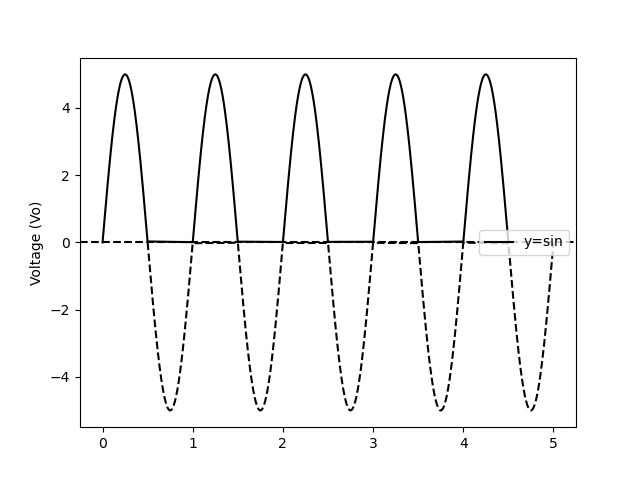
\includegraphics{figs/gate_25_fig5.png}
    \caption{Output Waveform}
    \label{fig:gate_ee_25_5}
\end{figure}

\begin{figure}[H]
    \centering
    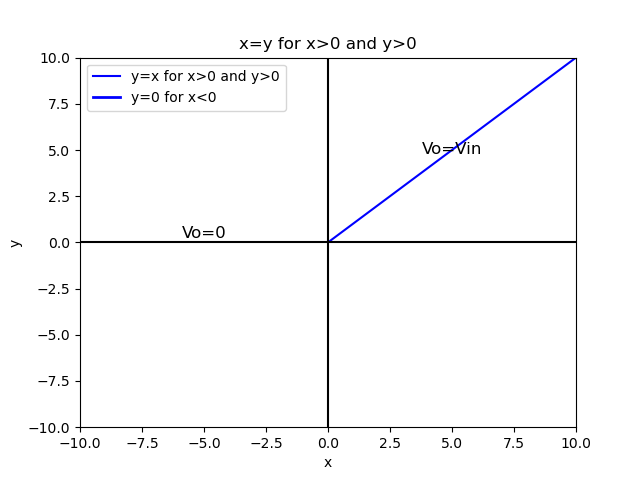
\includegraphics{figs/gate_25_fig6.png}
    \caption{charecterstic graph}
    \label{fig:gate_ee_25_6}
\end{figure}
The solution is Option A
\end{document}



\pagebreak

\item
Consider an FM broadcast that employs the pre-emphasis filter with frequency response \\
    \begin{align*}
        H_{pe}\brak{\omega}= 1+ \frac{j\omega}{\omega _0},
    \end{align*}
    where $\omega_0=10^4$ rad/sec. \\
    For the network shown in the figure to act as a corresponding de-emphasis filter, the
appropriate pair(s) of (R,C) values is/are 
\underline{\hspace{1in}} \\ \\
\begin{center}
    \begin{circuitikz}
		\draw
		(0,0)  to[resistor,*-,l=$R$] (4,0)
		to[capacitor,l=$C$] (4,-4) to (7,-4)
		(4,0) -- (7,0)
		(4,-4) to[short,-*] (0,-4);
		\node[below left] at (0,0){$+$};
		\node[above left] at (0,-4){$-$};
		\node[below right] at (7,0){$+$};
		\node[above right] at (7,-4){$-$};
		\draw [<->] (0,-0.3) -- (0,-3.7);
		\node[left] at (0,-2){input};
		\draw [<->] (7,-0.3) -- (7,-3.7);
		\node[right] at (7,-2){output};
	\end{circuitikz}
\end{center}
\begin{enumerate}
    \item[A.] $R=1k\ohm$, $C=0.1\micro F$
    \item[B.] $R=2k\ohm$, $C=1\micro F$
    \item[C.] $R=1k\ohm$, $C=2\micro F$
    \item[D.] $R=2k\ohm$, $C=0.5\micro F$
\end{enumerate} \\
\hfill(GATE EC 2022 51) \\
\solution
\iffalse
\let\negmedspace\undefined
\let\negthickspace\undefined
\documentclass[journal,12pt,onecolumn]{IEEEtran}
\usepackage{cite}
\usepackage{amsmath,amssymb,amsfonts,amsthm}
\usepackage{algorithmic}
\usepackage{graphicx}
\usepackage{textcomp}
\usepackage{xcolor}
\usepackage{txfonts}
\usepackage{listings}
\usepackage{enumitem}
\usepackage{mathtools}
\usepackage{gensymb}
\usepackage[breaklinks=true]{hyperref}
\usepackage{tkz-euclide} % loads  TikZ and tkz-base
\usepackage{listings}
\usepackage[siunitx]{circuitikz}[american voltages]
\usetikzlibrary{decorations.markings}

\newtheorem{theorem}{Theorem}[section]
\newtheorem{problem}{Problem}
\newtheorem{proposition}{Proposition}[section]
\newtheorem{lemma}{Lemma}[section]
\newtheorem{corollary}[theorem]{Corollary}
\newtheorem{example}{Example}[section]
\newtheorem{definition}[problem]{Definition}
%\newtheorem{thm}{Theorem}[section] 
%\newtheorem{defn}[thm]{Definition}
%\newtheorem{algorithm}{Algorithm}[section]
%\newtheorem{cor}{Corollary}
\newcommand{\BEQA}{\begin{eqnarray}}
\newcommand{\EEQA}{\end{eqnarray}}
\newcommand{\system}[1]{\stackrel{#1}{\rightarrow}}
\newcommand{\define}{\stackrel{\triangle}{=}}
\theoremstyle{remark}
\newtheorem{rem}{Remark}
%\bibliographystyle{ieeetr}
\begin{document}
%
\providecommand{\pr}[1]{\ensuremath{\Pr\left(#1\right)}}
\providecommand{\prt}[2]{\ensuremath{p_{#1}^{\left(#2\right)} }}        % own macro for this question
\providecommand{\qfunc}[1]{\ensuremath{Q\left(#1\right)}}
\providecommand{\sbrak}[1]{\ensuremath{{}\left[#1\right]}}
\providecommand{\lsbrak}[1]{\ensuremath{{}\left[#1\right.}}
\providecommand{\rsbrak}[1]{\ensuremath{{}\left.#1\right]}}
\providecommand{\brak}[1]{\ensuremath{\left(#1\right)}}
\providecommand{\lbrak}[1]{\ensuremath{\left(#1\right.}}
\providecommand{\rbrak}[1]{\ensuremath{\left.#1\right)}}
\providecommand{\cbrak}[1]{\ensuremath{\left\{#1\right\}}}
\providecommand{\lcbrak}[1]{\ensuremath{\left\{#1\right.}}
\providecommand{\rcbrak}[1]{\ensuremath{\left.#1\right\}}}
\newcommand{\sgn}{\mathop{\mathrm{sgn}}}
\providecommand{\abs}[1]{\left\vert#1\right\vert}
\providecommand{\res}[1]{\Res\displaylimits_{#1}} 
\providecommand{\norm}[1]{\left\lVert#1\right\rVert}
%\providecommand{\norm}[1]{\lVert#1\rVert}
\providecommand{\mtx}[1]{\mathbf{#1}}
\providecommand{\mean}[1]{E\left[ #1 \right]}
\providecommand{\cond}[2]{#1\middle|#2}
\providecommand{\fourier}{\overset{\mathcal{F}}{ \rightleftharpoons}}
\newenvironment{amatrix}[1]{%
  \left(\begin{array}{@{}*{#1}{c}|c@{}}
}{%
  \end{array}\right)
}
%\providecommand{\hilbert}{\overset{\mathcal{H}}{ \rightleftharpoons}}
%\providecommand{\system}{\overset{\mathcal{H}}{ \longleftrightarrow}}
	%\newcommand{\solution}[2]{\textbf{Solution:}{#1}}
\newcommand{\solution}{\noindent \textbf{Solution: }}
\newcommand{\cosec}{\,\text{cosec}\,}
\providecommand{\dec}[2]{\ensuremath{\overset{#1}{\underset{#2}{\gtrless}}}}
\newcommand{\myvec}[1]{\ensuremath{\begin{pmatrix}#1\end{pmatrix}}}
\newcommand{\mydet}[1]{\ensuremath{\begin{vmatrix}#1\end{vmatrix}}}
\newcommand{\myaugvec}[2]{\ensuremath{\begin{amatrix}{#1}#2\end{amatrix}}}
\providecommand{\rank}{\text{rank}}
\providecommand{\pr}[1]{\ensuremath{\Pr\left(#1\right)}}
\providecommand{\qfunc}[1]{\ensuremath{Q\left(#1\right)}}
	\newcommand*{\permcomb}[4][0mu]{{{}^{#3}\mkern#1#2_{#4}}}
\newcommand*{\perm}[1][-3mu]{\permcomb[#1]{P}}
\newcommand*{\comb}[1][-1mu]{\permcomb[#1]{C}}
\providecommand{\qfunc}[1]{\ensuremath{Q\left(#1\right)}}
\providecommand{\gauss}[2]{\mathcal{N}\ensuremath{\left(#1,#2\right)}}
\providecommand{\diff}[2]{\ensuremath{\frac{d{#1}}{d{#2}}}}
\providecommand{\myceil}[1]{\left \lceil #1 \right \rceil }
\newcommand\figref{Fig.~\ref}
\newcommand\tabref{Table~\ref}
\newcommand{\sinc}{\,\text{sinc}\,}
\newcommand{\rect}{\,\text{rect}\,}
%%
%	%\newcommand{\solution}[2]{\textbf{Solution:}{#1}}
%\newcommand{\solution}{\noindent \textbf{Solution: }}
%\newcommand{\cosec}{\,\text{cosec}\,}
%\numberwithin{equation}{section}
%\numberwithin{equation}{subsection}
%\numberwithin{problem}{section}
%\numberwithin{definition}{section}
%\makeatletter
%\@addtoreset{figure}{problem}
%\makeatother

%\let\StandardTheFigure\thefigure
\let\vec\mathbf


\bibliographystyle{IEEEtran}
\title{GATE-EC-51}
\author{EE23BTECH11059- Tejas Mehtre$^{*}$% <-this % stops a space
}
\maketitle




\bigskip

\renewcommand{\thefigure}{\theenumi}
\renewcommand{\thetable}{\theenumi}
%\renewcommand{\theequation}{\theenumi}
Consider an FM broadcast that employs the pre-emphasis filter with frequency response \\
    \begin{align*}
        H_{pe}\brak{\omega}= 1+ \frac{j\omega}{\omega _0},
    \end{align*}
    where $\omega_0=10^4$ rad/sec. \\
    For the network shown in the figure to act as a corresponding de-emphasis filter, the
appropriate pair(s) of (R,C) values is/are 
\underline{\hspace{1in}} \\ \\
\begin{center}
    \begin{circuitikz}
		\draw
		(0,0)  to[resistor,*-,l=$R$] (4,0)
		to[capacitor,l=$C$] (4,-4) to (7,-4)
		(4,0) -- (7,0)
		(4,-4) to[short,-*] (0,-4);
		\node[below left] at (0,0){$+$};
		\node[above left] at (0,-4){$-$};
		\node[below right] at (7,0){$+$};
		\node[above right] at (7,-4){$-$};
		\draw [<->] (0,-0.3) -- (0,-3.7);
		\node[left] at (0,-2){input};
		\draw [<->] (7,-0.3) -- (7,-3.7);
		\node[right] at (7,-2){output};
	\end{circuitikz}
\end{center}
\begin{enumerate}
    \item[A.] $R=1k\ohm$, $C=0.1\micro F$
    \item[B.] $R=2k\ohm$, $C=1\micro F$
    \item[C.] $R=1k\ohm$, $C=2\micro F$
    \item[D.] $R=2k\ohm$, $C=0.5\micro F$
\end{enumerate}
  \solution
  \fi
    \begin{table}[!ht]
    \centering
        \begin{tabular}{|c|c|c|} 
      \hline
\textbf{Variable}& \textbf{Description}& \textbf{Value}\\\hline
        $H_pre$& Frequency response of pre-emphasis filter & $1+\text{j}\frac{\omega}{\omega_0}$\\ \hline
        $\omega_0$ &Fundamental Frequency & $10^4$ rad/sec \\ \hline
    \end{tabular}
    \caption{input parameters}
    \label{}
\end{table}
\\
    Taking KVL around the loop,
    \begin{align}
        -V_i\brak{t} + i\brak{t}R + V_0\brak{t}=0 
    \end{align}
    \begin{align}
        \mathcal{L}\brak{f'\brak{t}} &\xleftrightarrow{\mathcal{L}} sF\brak{s}-f\brak{0} \label{q:2022/EC/51/1} \\
        i\brak{t}&= C\frac{dV_0\brak{t}}{dt} \label{eq:2022/EC/51/2}
    \end{align}
    Using \eqref{q:2022/EC/51/1} and \eqref{eq:2022/EC/51/2},
    \begin{align}
        \mathcal{L}\brak{ -V_i\brak{t} + RC\frac{dV_0\brak{t}}{dt} + V_0\brak{t}}&=\mathcal{L}\brak{0} \\
        V_0\brak{s}\brak{1+j\omega RC}&= V_i\brak{s} \\
         H\brak{j\omega}=\frac{V_o\brak{j\omega}}{V_i\brak{j\omega}} &= \frac{1}{1+j\omega RC}
    \end{align}
The given $RC$ circuit to act as de-emphasis filter
\begin{align}
    \abs{H\brak{j\omega}}&= \frac{1}{\abs{H_{pre}\brak{\omega}}} \\
    \frac{1}{\sqrt{1+\brak{\omega RC}^2}}&= \frac{1}{\sqrt{1+\brak{\frac{\omega}{\omega_0}}^2}} \\
    \omega_0&= \frac{1}{RC} \\
    \omega_0&=10^4 rad/sec
\end{align}
Thus $\omega_0=10^4$ rad/sec only possible if we choose $R=1k\ohm$ and $C=0.1\micro F$ from options. Hence, the correct option is (B).
\begin{figure}[ht]
        \centering
        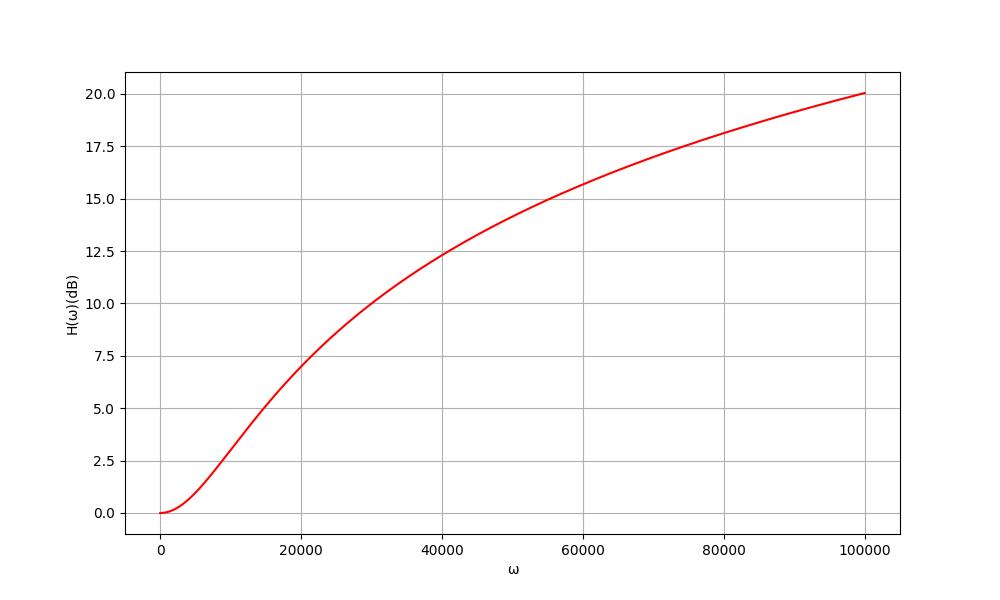
\includegraphics[width=\columnwidth]{2022/EC/51/figs/plot.png}
        \caption{Frequency response of a pre-emphasis filter.}
    \end{figure}

\pagebreak

\end{enumerate}
